\documentclass[]{abnt}
\usepackage[T1]{fontenc}
\usepackage[latin1]{inputenc}
\usepackage[brazil]{babel}
\usepackage{amsthm,amsmath,amssymb}
\usepackage{float}
\usepackage{color}
\usepackage{fancyhdr}
\usepackage{hyperref}
\usepackage{graphicx}
% \usepackage{lastpage}
\usepackage{setspace}
\usepackage[caixa=Mm,paginas=nao,ordem=alf]{tabela-simbolos}
\usepackage[alf,abnt-etal-list=3,abnt-url-package=hyperref]{abntcite} % Se >3 autores, entao usar et al.

\newtheorem*{teorema}{Teorema}
\newcommand{\unificar}{\ensuremath{\mathit{unificar\/}}}

\begin{document}

% estilos.tex

% Faz a linha da \assinatura aparecer, o valor padrao eh 0pt
\setlength{\ABNTsignthickness}{0.4pt}

% Muda o marcador do itemize para hifen, ao inves da bolinha preenchida
%\RequirePackage{atbeginend}
%\AfterBegin{itemize}{\addtolength{\itemsep}{-0.5em}}
\renewcommand{\labelitemi}{--}


% declaracoes.tex

\hyphenation{gra-m�-ti-ca}

\onehalfspacing

% newcommands

\newcommand{\ingles}[1]{\textsl{#1}}

\newcommand{\progb}[1]{
  \normalfont\ttfamily 
  {\small 
  \begin{center}
  \parbox{\textwidth}{\begin{tabbing}
        #1 
  \end{tabbing}}
  \end{center} }
  \normalfont}

\newcommand{\progfig}[1]{\fbox{\parbox{\textwidth}{
  \normalfont\ttfamily 
  {\small 
  \begin{center}
  \parbox{\textwidth}{\begin{tabbing}
        #1 
  \end{tabbing}}
  \end{center} }
  \normalfont}}}


\autor{Adriano Bonat Alves}
\titulo{Compilando c�digo funcional para bytecodes Java}
\orientador{Prof. Dr. Cristiano Damiani Vasconcelos}
\instituicao{Universidade Federal de Pelotas - UFPel}
\local{Pelotas}
\data{Novembro de 2008}

\capa
\folhaderosto

%\begin{folhadeaprovacao}
%	\assinatura{Prof. Dr. Cristiano Damiani Vasconcelos \\ Orientador}
%	\assinatura{Prof. Dr. Fulano de Tal}
%\end{folhadeaprovacao}

% resumo.tex
\begin{resumo}

\noindent
ALVES, Adriano B. \textbf{Compilando c�digo funcional para \textit{bytecodes} Java}. 2008. 73f.
Trabalho acad�mico (Gradua��o) -- Bacharelado em Ci�ncia da Computa��o. Universidade Federal de Pelotas, Pelotas.
\\

\onehalfspacing

\noindent
Este trabalho prop�e o estudo da interoperabilidade e dos problemas envolvidos na tradu��o entre 
linguagens de diferentes paradigmas, principalmente entre os paradigmas funcional e orientado a objeto.
Para a realiza��o deste estudo, foi desenvolvido um compilador de uma linguagem funcional que gera
\textit{bytecodes} Java.
A interoperabilidade entre linguagens � de grande interesse, como mostra o sucesso das plataformas .NET
e Java, respectivamente da Microsoft e da Sun Microsystems.
Um dos motivos da baixa ado��o de linguagens funcionais � a falta de uma maneira f�cil destas interoperarem
com outras linguagens.
A m�quina virtual Java executa programas bin�rios na forma de \textit{bytecodes} Java. 
Embora esta m�quina virtual tenha sido desenvolvida para a linguagem de programa��o Java, outras linguagens 
de programa��o podem ser executadas sobre esta.
Alguns dos motivos do grande interesse por m�quinas virtuais s�o a explos�o da web, grandes sistemas
desenvolvidos com base em v�rias linguagens e o suporte a c�digo legado. A m�quina virtual resolve estes
problemas, pois � uma plataforma onde v�rias linguagens podem interoperar.
A linguagem funcional definida neste trabalho tem sintaxe similar a de Haskell,
sua ordem de avalia��o � estrita,
� estaticamente tipada, possui infer�ncia de tipos e n�o possui suporte � sobrecarga (\textit{overload}).
\\

\noindent
Palavras-chave: Sistema de tipos. Linguagens funcionais. Interoperabilidade. Orienta��o a objeto.
\end{resumo}


% abstract.tex
\begin{englishabstract}{Compilando c�digo funcional para bytecodes Java}{Type system, functional languages, interoperability, object oriented}

This work proposes the study of interoperability and problems involved in the translation between 
languages from different paradigms, particularly the functional paradigm and the object oriented.
For this study, was developed a compiler of a functional language that generates Java bytecodes. 
The interoperability between languages is of great interest, as demonstrated by the success of the platforms .NET 
and Java, respectively of Microsoft and Sun Microsystems. 
One of the reasons for the low adoption of functional languages is the lack of an easy way these interoperate 
with other languages. 
The Java virtual machine runs programs in a binary form called Java bytecodes. 
Although this virtual machine has been developed for the Java programming language, other programming
languages can benefit themselves too.
Some of the reasons for the great interest in virtual machines are the explosion of the web, the development
of large systems based on several languages and the support for legacy code. The virtual machine solves these 
problems because it is a platform where different languages can interoperate. 
The functional language defined in this work is similar to the syntax of Haskell, 
is strict, statically typed, has type inference and does not have support to overload.

\end{englishabstract}


\listoffigures
\listoftables
\listadesiglas

\sumario

% introducao.tex
\chapter{Introdu��o}

As primeiras linguagens de programa��o foram desenvolvidas com o simples objetivo de poder controlar
o comportamento dos computadores. Prova disto � que estas linguagens ofereciam diretamente, de uma forma
n�o abstrata, as funcionalidades do \textit{hardware} em que iriam ser executadas.

Desta forma, de linguagens de montagem primitivas surgiram v�rias linguagens de alto n�vel, come�ando com 
FORTRAN \cite{fortran} em 1950. O n�mero destas linguagens cresceu t�o rapidamente que no in�cio de 1980, para
um melhor estudo, estas j� eram agrupadas, devido �s suas semelhan�as, em fam�lias de linguagens \cite{hudak89}.

A fam�lia de linguagens de programa��o funcionais, na qual a computa��o � o resultado da avalia��o de express�es 
(principalmente a aplica��o de fun��es), tem atra�do, atualmente, a aten��o de pesquisadores tanto da �rea
acad�mica como da ind�stria de desenvolvimento de \textit{software}.

Uma das raz�es dessa atra��o, principalmente pelas linguagens funcionais puras e de avalia��o pregui�osa,
� que estas podem usufruir do poder de processamento dos processadores com m�ltiplos n�cleos (processadores
\textit{multicore}) \cite{meijer2008}. 
O fato de serem puras diz respeito � aus�ncia de efeito colateral, ou seja, a avalia��o
de uma express�o n�o influi no resultado da avalia��o de outra express�o. Juntamente com isso, o fato de 
ter uma avalia��o pregui�osa permite que a avalia��o dos par�metros de uma express�o seja realizado somente
quando necess�rio. Essas caracter�sticas fazem com que programas nestas linguagens sejam muito mais facilmente
paraleliz�veis do que em linguagens de paradigma imperativo \cite{hudak89}.

Embora as linguagens funcionais resolvam v�rios problemas, estas muitas vezes necessitam utilizar a interface
de fun��es externas (\textit{Foreign Function Interface} - FFI\sigla{FFI}{\textit{Foreign Function Interface} - Interface de fun��es externas}) para acessar alguma funcionalidade de que
n�o disp�em, como uma biblioteca de outra linguagem, ou ter acesso direto a servi�os do sistema operacional.
A import�ncia de boas FFIs � largamente reconhecida atualmente, principalmente
frente � tend�ncia de desenvolvimento baseado em componentes escritos em v�rias linguagens \cite{benton1999}.

Geralmente as linguagens funcionais possuem alguma maneira de chamar fun��es externas em C, por�m, trabalhar
diretamente com uma linguagem de mais baixo n�vel, que n�o tenha um sistema de tipos seguro e sem um coletor
de lixo nunca ir� ser trivial ou elegante \cite{benton1999}. 
Um dos motivos da baixa ado��o de linguagens funcionais � a falta de uma maneira f�cil destas interoperarem
com outras linguagens \cite{smlj}.

A interoperabilidade entre linguagens � de grande interesse, como mostra o sucesso das plataformas .NET
e Java, respectivamente da Microsoft e da Sun Microsystems. Os projetistas de linguagens de programa��o
demonstram isto atrav�s de linguagens como SML$\sharp$, Mondrian e Scala \cite{smlnet,mondrian,scala}. 
Todas estas linguagens
t�m a interoperabilidade com outras linguagens como sua funcionalidade principal \cite{matthews2007}.
Alguns dos motivos do grande interesse por m�quinas virtuais s�o a explos�o da web, grandes sistemas
desenvolvidos com base em v�rias linguagens e o suporte a c�digo legado. A m�quina virtual resolve estes
problemas, pois � uma plataforma onde v�rias linguagens podem interoperar.

A possibilidade de escrever algoritmos de forma concisa, ou ent�o facilmente paralelizar a execu��o 
destes algoritmos, demonstra alguns dos maiores poderes das linguagens funcionais.
Atrav�s da execu��o de uma linguagem funcional sobre a arquitetura de uma m�quina virtual
poder�amos obter os benef�cios da portabilidade, de termos um sistema
de tipos comum entre as linguagens, assim como tamb�m a seguran�a proporcionada pela \textit{sandbox}, que
protege o sistema hospedeiro durante a execu��o do programa.

\section{Motiva��o}

Como vimos na se��o anterior, � crescente o n�mero de linguagens de programa��o que baseiam a sua execu��o 
sobre m�quinas virtuais. Sobre a m�quina virtual Java temos como exemplo os projetos para rodar Python (Jython) \cite{jython}, Ruby (JRuby) \cite{jruby}, recentemente Scala, e centenas de outras linguagens \cite{jvmlangs}.

A m�quina virtual Java \cite{jvmspec} executa programas bin�rios na forma de \textit{bytecodes} Java. 
Embora esta m�quina virtual tenha sido desenvolvida para a linguagem de programa��o Java, outras linguagens 
de programa��o podem ser executadas sobre esta.

A plataforma Java foi escolhida por diversas raz�es, dentre elas:

\begin{itemize}
	\item h� pouco tempo teve seu c�digo-fonte aberto, sendo poss�vel para qualquer pessoa estud�-lo;
	\item a m�quina virtual Java � uma das mais populares;
	\item a linguagem Java � a mais popular\footnote{O �ndice da comunidade de programa��o TIOBE leva em conta o n�mero de pessoas que utilizam a linguagem, assim como o n�mero de cursos e de parceiros (\textit{third party vendors}).} segundo TIOBE \cite{tiobe}, sendo mais popular que a linguagem C.
\end{itemize}

O prop�sito deste trabalho � o desenvolvimento de uma base que possibilite futuras pesquisas sobre a 
interoperabilidade entre linguagens de diferentes paradigmas, principalmente entre os paradigmas funcional 
e orientado a objeto.
Como parte dessa base, foi desenvolvido um compilador de uma linguagem funcional que gera
\textit{bytecodes} Java.

\section{Objetivos}

O objetivo deste trabalho � implementar um compilador que permita o estudo dos problemas envolvidos na gera��o
de c�digo funcional para a m�quina virtual Java, assim como a interoperabilidade entre as linguagens
do paradigma funcional e orientado a objeto.
Essa implementa��o envolve:

\begin{itemize}
	\item a defini��o de uma linguagem funcional estrita e sem sobrecarga, baseada na sintaxe de Haskell;
	\item a constru��o de um compilador, onde o \textit{frontend} � composto por um analisador sint�tico e 
um inferidor de tipos, e cujo \textit{backend} gera \textit{bytecodes} Java;
	\item o estudo dos poss�veis problemas de interoperabilidade entre o paradigma funcional e o orientado
a objeto.
\end{itemize}

Em rela��o a gera��o de c�digo, ser�o abordadas apenas as representa��es de tipos de dados alg�bricos
e um estudo inicial sobre a tradu��o de fun��es.

\section{Organiza��o do Trabalho}

Este trabalho, dividido em cinco cap�tulos, apresenta primeiramente os conceitos estudados durante o seu
desenvolvimento, seguido da descri��o da ferramenta desenvolvida, os resultados obtidos e as conclus�es.

No cap�tulo dois, � apresentada uma introdu��o � programa��o funcional, suas caracter�sticas, como
funciona a infer�ncia de tipos, e tamb�m um pouco da evolu��o das linguagens deste paradigma de desenvolvimento
de \textit{software}.

O cap�tulo tr�s trata da m�quina virtual Java, descrevendo suas caracter�sticas, \textit{opcodes}, tipos de
dados, modelo de execu��o e tamb�m sobre seus arquivos de \textit{bytecodes} (arquivos \textit{.class}).

No quarto cap�tulo, � descrita a ferramenta desenvolvida, as bibliotecas utilizadas e
as tradu��es feitas entre as express�es da linguagem funcional deste trabalho para constru��es 
na linguagem Java.

No quinto e �ltimo cap�tulo, s�o apresentadas as conclus�es e as sugest�es de trabalhos futuros.


% capitulo1.tex
\chapter{Programa��o Funcional}

Programa��o Funcional � assim chamada porque um programa consiste inteiramente em fun��es. A pr�pria fun��o
principal do programa � definida em termos de outras fun��es, e assim sucessivamente, at� o n�vel base das
fun��es, que s�o as primitivas da linguagem \cite{whyfp}. Ao contr�rio do paradigma imperativo, linguagens
funcionais, em sua forma pura, n�o suportam mudan�as de estado, dando �nfase na aplica��o de fun��es.

Este cap�tulo mostra as origens da programa��o funcional com o C�lculo Lambda na se��o \ref{sec:calclambda},
e nas se��es seguintes explora as primeiras linguagens funcionais e a evolu��o delas at� a linguagem estado
da arte, Haskell, na se��o \ref{sec:haskell}.

\section{C�lculo Lambda}
\label{sec:calclambda}

O c�lculo lambda � um modelo matem�tico, e pode ser pensado como uma linguagem de programa��o pura, baseada 
na defini��o e aplica��o de fun��es, e o seu m�todo de itera��o � atrav�s da recurs�o. Esse modelo permite 
a representa��o de qualquer algoritmo, e � pura no sentido de que as fun��es recebem e retornam dados, que 
podem ser inclusive fun��es, e n�o podem ser alterados pela fun��o.

Na �rea da matem�tica e da ci�ncia da computa��o, fun��es de ordem superior (\textit{high order functions}) s�o fun��es que podem receber fun��es como argumentos, assim como produzir fun��es como resultado de sua
computa��o.

Por ser um modelo simples, o c�lculo lambda permite demonstrar alguns conceitos importantes de linguagens de programa��o, como por exemplo liga��o, escopo, ordem de avalia��o, computabilidade, sistemas de tipos, etc.

Existem tr�s tipos de express�es lambda:

\begin{itemize}
	\item Vari�veis: expressas, normalmente, atrav�s de identificadores alfan�mericos;
	\item Aplica��es ($e_1$ $e_2$): representam a aplica��o da express�o $e_1$ para $e_2$;
	\item Abstra��es ($\lambda{}x.e$): representam a fun��o que retorna o valor $e$ quando recebe o par�metro formal $x$.
\end{itemize}


Podemos, por exemplo, definir a fun��o identidade atrav�s da seguinte \textit{abstra��o-$\lambda{}$}:

\begin{center}
$(\lambda{}x. x)$
\end{center}

Quando as abstra��es-$\lambda{}$ encontram-se aninhadas, h� a conven��o sint�tica de deixar de usar 
o ponto para separ�-las, assim como de eliminar os par�nteses para facilitar o entendimento 
da express�o. Outras duas conven��es dizem respeito quanto � ordem de aplica��o das fun��es, que devem
ocorrer da esquerda para a direita, e que o escopo de uma abstra��o-$\lambda{}$ se estende o m�ximo
poss�vel para a direita, por exemplo $\lambda{}x.xy$ deve ser lido como $\lambda{}x.(xy)$, e n�o como
$(\lambda{}x.x)y$. Em uma express�o $\lambda{}x.E$, $E$ � chamado de escopo $x$.

As vari�veis em express�es-$\lambda{}$ podem ser \textit{ligadas} ou \textit{livres}. Uma vari�vel � ligada
quando est� associada a uma abstra��o-$\lambda{}$, e livre caso contr�rio.
Express�es que diferem apenas no nome das vari�veis ligadas (ou seja, n�o h� uma diferen�a sem�ntica)
s�o chamadas de express�es $\alpha{}$-equivalentes, por exemplo a express�o $(\lambda{}y. y)$ �
$\alpha{}$-equivalente � fun��o identidade mostrada previamente, logo s�o express�es sin�nimas.

A aplica��o de abstra��es-$\lambda{}$ � baseada em substitui��es, por exemplo:

\progb{
	$(\lambda{}x.M)N = [N/x]M$
}

\noindent
significa que $N$ � o par�metro da abstra��o-$\lambda{}$. Assim, todas as ocorr�ncias de $x$
na express�o $M$ ser�o substitu�das pela express�o $N$, e essa substitui��o pode ser representada
por $[N/x]M$. Uma express�o $W$ � dita $\beta{}$-equivalente a $Y$ se a express�o $W$ for
$\alpha{}$-equivalente a $Y$ ap�s zero ou mais substitui��es.
As seguintes express�es s�o $\beta{}$-equivalentes a $x$:

\progb{
	$(\lambda{}y.y)x$ \\
	$(\lambda{}y.x)x$ \\
	$(\lambda{}f.f x)(\lambda{}y.y)$ \\
	$x$
}

Em c�lculo lambda h� duas ordens de se avaliar uma express�o: avalia��o por valor (\textit{eager evaluation}),
onde a redu��o ocorre no par�metro antes deste ser aplicado � fun��o, e \label{sec:avpreguicosa} avalia��o pregui�osa (\textit{lazy evaluation}), onde o par�metro da fun��o � substitu�do inteiramente no corpo da fun��o, havendo redu��o do par�metro dentro do corpo da fun��o somente se necess�rio.

A ordem de avalia��o de uma express�o � importante, pois pode resultar na express�o na sua forma normal
(quando nenhuma substitui��o pode mais ser aplicada a uma express�o), ou ent�o no n�o t�rmino da computa��o.
A express�o $(\lambda{}x\lambda{}y.y)((\lambda{}z.zz)(\lambda{}z.zz))(\lambda{}w.w)$ demonstra a import�ncia
da escolha da ordem de avalia��o, uma vez que atrav�s da ordem de avalia��o por valor a computa��o dessa
express�o n�o terminaria.

% Watt, D. A. (1991). Programming Languages Syntaxe and Semantics. Prentice Hall
\parbox{14.5cm}{
\textbf{Teorema de Church e Rosser}:
Se $v$ � o resultado da avalia��o de uma
express�o $M$ aplicando a ordem de avalia��o pregui�osa, ent�o qualquer
que seja a ordem aplicada, ou o resultado � $v$ ou a avalia��o falha (n�o termina).
Se a avalia��o de $M$ n�o termina usando a ordem pregui�osa, a avalia��o 
n�o termina usando qualquer ordem. \cite{ChurchRosser36}
}

\section{LISP}
LISP ou Lisp \cite{Mc65} \sigla{Lisp}{\textit{LISt Processor} - Processador de listas} (acr�nimo para \textit{LISt Processor}) foi a primeira linguagem de programa��o
a possibilitar a defini��o de express�es sem efeitos colaterais \cite{jmitchell2003}.
O projeto da linguagem foi publicado por McCarthy em um artigo em 1960 \cite{Mc60}, onde mostrava que com apenas
alguns simples operadores e uma nota��o para fun��es, era poss�vel construir uma linguagem Turing-completa
\cite{wikipediaLisp}. Sua principal aplica��o � na �rea de pesquisa em intelig�ncia artificial e computa��o
simb�lica.

Muitas implementa��es de Lisp foram desenvolvidas, levando a diversos dialetos da linguagem,
como o Maclisp desenvolvido no MIT na d�cada de 1960, e o Scheme, desenvolvido tamb�m no MIT na
d�cada de 1970 por Guy Steele e Gerald Sussman. Atualmente a forma de Lisp mais usada �
o \textit{Common Lisp} \cite{IPS:1994:DPA}, que � uma especifica��o da linguagem publicada pela ANSI, e
cont�m algumas primitivas de orienta��o a objeto.

Embora Lisp tenha sua inspira��o no c�lculo lambda, elas possuem algumas diferen�as importantes.
Listas s�o o principal tipo de dado de Lisp, enquanto fun��es s�o o �nico tipo de dado no c�lculo
lambda puro (existe o c�lculo lambda enriquecido, que possui algumas constru��es como de sele��o,
que tornam o uso de c�lculo lambda mais agrad�vel e f�cil).

Na especifica��o original, existia apenas dois tipos de dados: �tomos e listas. �tomos podem ser
alfan�mericos ou apenas n�meros, e sua diferen�a consiste em ser imut�vel e �nico. As listas em Lisp s�o
simplesmente ligadas, sendo a fun��o $car$ usada para retornar o dado do nodo, e $cdr$ para retornar
o pr�ximo nodo. A fun��o $cons$ � utilizada para construir uma lista, e existe a lista vazia,
denotada por $nil$.

O artigo de McCarthy definia duas sintaxes poss�veis para a linguagem: express�es-S (\textit{s-expressions}
ou \textit{Symbolic expressions}) e express�es-M (\textit{Meta expressions}), embora a segunda n�o seja muito usada.
Express�es-S representam listas, e misturam c�digos e dados em uma representa��o
regular, baseada no uso intensivo de par�nteses, que representam listas, e tem como o espa�o o separador
dos elementos. Desta forma, a linguagem � extremamente flex�vel, pois fun��es s�o declaradas como listas, 
e assim podem ser processadas uniformemente como se fossem dados, o que d� origem � id�ia de \textit{meta-programa��o}, onde programas podem se modificar.

Lisp, na verdade, n�o � uma linguagem totalmente pura. Apenas um sub-conjunto de suas fun��es � puro,
o que forma o chamado Lisp puro. S�o elas:

\begin{tabular}{ll}
	$cons$ & constr�i uma lista \\
	$car$ & retorna o dado do nodo \\
	$cdr$ & retorna o pr�ximo nodo \\
	$eq$ & retorna $true$ se as duas express�es t�m o mesmo valor \\
	$atom$ & retorna $true$ se o valor da express�o � at�mico
\end{tabular}

\noindent
e algumas fun��es especiais:

\begin{tabular}{ll}
	$cond$ & retorna o valor da primeira express�o que tiver valor diferente de $nil$ \\
	$lambda$ & similar ao c�lculo lambda, retorna uma express�o para ser avaliada \\
	$define$ & associa um �tomo a uma express�o \\
	$quote$ & retorna uma express�o cujo valor � o seu par�metro \\
	$eval$ & avalia o seu par�metro \\
\end{tabular}

As express�es que come�am com alguma dessas fun��es especiais s�o avaliadas de tal forma que determinadas
partes de sua express�o n�o ir�o ser avaliadas naquele momento, por exemplo:

\progb{
	($cond$ ($p_1$ $e_1$) ($p_2$ $e_2$) ($p_n$ $e_n$))
}

Na express�o exemplificada, a avalia��o dos par�metros de $cond$ vai ocorrer da esquerda para a direita, 
achando o primeiro $p_i$ com valor diferente de $nil$, retornando ent�o o valor da express�o $e_i$.

\progb{
	(($lambda$ ($x$) ($+$ $x$ $10$)) $8$)
}

Nesse exemplo da fun��o $lambda$, os seus par�metros s� ser�o avaliados quando um valor for aplicado.
Se executada, essa express�o possui o valor $18$.

  \progb{
   ($define$\={} $find$ ($lambda$ ($x$ $y$) \\
     \>($cond$\={} (($eq$ $y$ $nil$) $nil$)   \\
     \>\>     (($eq$ $x$ ($car$ $y$)) $x$)  \\
     \>($true$ ($find$ $x$ ($cdr$ $y$)))  \\
   )))
  }

Atrav�s desse exemplo � mostrado como ocorre a recurs�o em Lisp, onde associamos ao �tomo $find$ 
uma express�o lambda. A fun��o $find$ procura um elemento $x$ em uma lista $y$,
retornando o valor $x$ caso o encontre, ou ent�o retorna $nil$ caso o elemento $x$ n�o seja
encontrado na lista.

\section{ML}
\label{sec:ML}

A fam�lia de linguagens baseada em Algol foi desenvolvida em
paralelo com Lisp, e levou ao desenvolvimento de ML e Modula \cite{Wirth77}.

As principais caracter�sticas das linguagens derivadas de Algol
s�o as express�es separadas por ponto e v�rgula, a estrutura em blocos,
fun��es e procedimentos, e tipagem est�tica.

ML foi a primeira linguagem a incluir infer�ncia de tipos polim�rficos.

ML � uma linguagem funcional com algumas possibilidades imperativas, sendo por isso
considerada uma linguagem funcional impura.
Ao mesmo tempo que � poss�vel criar fun��es atrav�s de express�es lambda,
pass�-las para outras, e retornar fun��es como resultado
de computa��es, ML tamb�m permite a escrita de algoritmos de forma imperativa,
com uma sintaxe parecida com a de linguagens que descendem da fam�lia Algol.
A vers�o de ML mais utilizada � a \textit{Standard} ML \cite{Mil90}.

Enquanto Lisp � uma linguagem dinamicamente tipada, ou seja, os tipos das express�es
s�o resolvidos em tempo de execu��o, ML � uma linguagem estaticamente
tipada, onde as express�es possuem seus tipos resolvidos em tempo de compila��o. 
Seu sistema de tipos foi parte importante
do projeto da linguagem, e � frequentemente considerado o mais limpo e expressivo 
\cite{jmitchell2003}.

At� o desenvolvimento do sistema de tipos de ML, linguagens com sistemas de tipos consistentes 
(\textit{sound type systems})
eram consideradas restritivas. Esse novo sistema � matematicamente preciso, no sentido
de que se uma parte do compilador, chamado de verificador de tipos (\textit{type checker}), determina que uma express�o
possui um certo tipo, � ent�o garantido que na avalia��o daquela express�o o valor resultante ter� como tipo
o mesmo determinado pelo verificador. Logo, uma das vantagens que linguagens estaticamente tipadas
possuem � essa seguran�a dada pelo verificador de tipos, que possibilita que v�rios problemas de programa��o
sejam encontrados em tempo de compila��o. Por exemplo, se o verificador determinou que uma express�o possui
o tipo ``ponteiro para string'', ent�o � garantido que quando a express�o for avaliada, o valor dessa express�o
ser� um ``ponteiro para string'', e n�o um ponteiro para uma string que j� foi desalocada da mem�ria, ou que
esteja apontando para outro valor que n�o uma string.

A linguagem foi desenvolvida por Robin Milner e seus colegas na d�cada de 1970 na Universidade de Edinburgh,
como parte de um projeto maior chamado de \textit{Logic for Computable Functions} - LCF \sigla{LCF}{\textit{Logic for Computable Functions} - L�gica para fun��es comput�veis}, cujo objetivo era desenvolver
um sistema para provar propriedades de programas funcionais, de uma maneira autom�tica ou semi-autom�tica.
Dessa maneira, ML foi desenvolvida como uma meta-linguagem (da� a origem de seu nome, \textit{Meta-language})
 para o projeto LCF.
\sigla{ML}{\textit{Meta-language} - Meta linguagem}

Um conceito fundamental do LCF � o de t�ticas de prova (\textit{proof tatics}), que consiste em uma fun��o
que recebe uma f�rmula, e realizando algumas asser��es tenta achar uma prova para essa f�rmula.
Essa fun��o possui tr�s poss�veis resultados:

\parbox{\textwidth}{\[ t\acute{a}tica(f\acute{o}rmula) = \left\{ \begin{array}{l}
	\text{tem sucesso e retorna a prova} \\
	\text{procura infinitamente} \\
	\text{falha}
\end{array}\right.
\]
}

Uma id�ia adotada foi desenvolver um tipo $prova$, que seria retornado pela fun��o \textit{t�tica},
e distinguiria os resultados onde se consegue uma prova para a f�rmula dos que n�o conseguem.
Assim o tipo da fun��o seria:

\begin{center}
	\textit{t�tica}: \textit{f�rmula} $\rightarrow{}$ \textit{prova}
\end{center}

O problema que surgiu dessa solu��o foi como retornar as situa��es de falha pela fun��o. Milner
desenvolveu ent�o o primeiro mecanismo de exce��es com tipagem segura (\textit{type-safe}). Desse modo,
quando for detectado que n�o h� uma prova para a f�rmula, a fun��o pode lan�ar uma exce��o.

Com esse mecanismo de exce��es em ML, a nota��o:

\begin{center}
	$f$: $A$ $\rightarrow{}$ $B$
\end{center}

significa $\forall{}x$ em $A$, se $f(x)$ termina normalmente sem lan�ar uma exce��o, ent�o
$f(x)$ est� em $B$.

\subsection{Declara��es e Tipos de Dados}

Em ML as declara��es que associam o valor de uma express�o a um identificador s�o escritas
da seguinte maneira:

\progb{
	val <identificador> = <express�o>;
}

Assim, se quis�ssemos associar o valor $3$ ao identificador $y$, far�amos:

\progb{
	val y = 3;
}

� importante notar que uma vez associado um valor a um identificador, esse n�o muda, portanto
as declara��es de ML introduzem constantes, n�o vari�veis.

H� duas maneiras de se declarar fun��es, uma com sintaxe uniforme com a declara��o
de identificadores, e que de certa forma lembra c�lculo lambda:

\progb{
	val f = fun x => x+1;
}

\noindent
e outra que n�o utiliza de atribui��o:

\progb{
	fun f(x) = x + 1;
}

\noindent
por�m ambas as declara��es se comportam da mesma maneira quando executadas. Na realidade o compilador
transforma a segunda forma na primeira, sendo assim apenas um ``a��car sint�tico''
\footnote{A��car sint�tico (\textit{syntatic sugar}) � um termo introduzido por Peter Landin, que significa adi��es a sintaxe
de uma linguagem de programa��o que n�o afetam a sua funcionalidade, apenas tornam o seu uso mais
agrad�vel (em ingl�s \textit{sweeter}) ao programador}.

\subsubsection{Tipos B�sicos}

Os seguintes tipos b�sicos fazem parte de ML:

\begin{itemize}
	\item \textit{Unit}
	\progb {() : unit}
	Assim como o \textit{void} da linguagem C \cite{Ker88}, � o tipo de retorno de fun��es
	que realizam apenas efeitos colaterais.
	
	\item \textit{Bool} \\
	\progb{true : bool \\ false : bool}
	Possui apenas esses dois valores v�lidos, sendo que valores $booleanos$ est�o geralmente
	associados � estrutura de sele��o $if$:
	
	\progb{
		if $e_1$ then $e_2$ else $e_3$
	}
	
	sendo que a express�o $e_1$ deve ser um $booleano$, e $e_2$ e $e_3$ devem possuir o mesmo tipo, j�
	que o resultado de um $if$ � a execu��o de $e_2$ ou $e_3$, e este � o tipo da express�o $if$.
	
	Existem tamb�m as opera��es $AND$, $OR$ e $NOT$, por�m o nome dos dois primeiros s�o $andalso$ e
	$orelse$, nomes que refor�am qual � a ordem de avalia��o. Por exemplo em uma express�o $a$ $andalso$ $b$,
	se a express�o $a$ for $true$ ent�o $b$ ser� avaliado, caso contr�rio n�o. J� na express�o 
	$a$ $orelse$ $b$, caso $a$ seja $true$ a express�o $b$ n�o ser� avaliada.
	
	\item Inteiros \\
	Valores como $-2,-1,0,1,2$ s�o inteiros v�lidos em ML, e possuem as seguintes opera��es aritm�ticas
	triviais dispon�veis: $+$, $-$, $*$ e $div$. Esses operadores s�o usados na forma infixa.
	
	\item Strings \\
	S�o representadas atrav�s de uma sequ�ncia de caracteres entre aspas duplas.
	\progb{``Ol� mundo!'' :  string}
	
	\item Real \\
	O tipo para n�meros de ponto-flutuante em ML � o $real$, e as opera��es aritm�ticas $+$, $-$ e $*$ s�o
	sobrecarregadas, por�m operam apenas com operandos do mesmo tipo. Por exemplo, a soma de um n�mero
	inteiro $7$ e o n�mero $5,2$ � inv�lida, pois s�o de tipos diferentes. Para essa soma ocorrer,
	o n�mero $7$ poderia ser convertido para ponto-flutuante atrav�s da fun��o $real$, ou ent�o utilizar
	as fun��es $ceil$ (arredonda para cima) ou $floor$ (arredonda para baixo) para converter o n�mero $5,2$.
	
	\item Tuplas \\
	As tuplas podem ser de dois, tr�s, \ldots{} $n$ tipos distintos:
	
	\progb{
		(256, ``Maria'') \\
		('Nitrog�nio, 14.00674, ``N�o metal'')
	}

	Partes da tupla podem ser acessadas atrav�s de fun��es que iniciam com ``\#'' e s�o seguidas
	pela posi��o da parte desejada, que come�a em 1. Por exemplo: $\#1(256$, $``Maria'')$ retornaria
	o n�mero $256$.
	
	\item Registros \\
	Assim como os registros em Pascal \cite{Wir91}, ou \textit{structs} em C, em ML existem os chamados registros,
	que s�o parecidos com as tuplas, por�m usam ap�strofos ao inv�s de par�nteses e as partes possuem nomes:
	
	\progb{
		val pessoa = \{ Nome = ``Alfredo'', Idade = 33 \}
	}
	
	O m�todo para acessar alguma parte do registro � tamb�m parecido com o de tuplas. Utiliza-se, por exemplo, 
	$\#Nome(pessoa)$ para acessar o campo correspondente ao nome da $pessoa$.
	
	\item Listas \\
	As listas em ML podem ter qualquer tamanho, com a restri��o de que todos os elementos da lista possuam
	o mesmo tipo de dados. A lista vazia em ML, assim como em Lisp, � representada por $nil$, e a fun��o
	$cons$ por dois pontos.

	\progb{
		$3$ :: $nil$ \\
		$1$ :: $2$ :: $[3$,$4$,$5]$
	}
	
	O primeiro exemplo constr�i a lista $[3]$, enquanto o segundo a lista $[1,2,3,4,5]$.
\end{itemize}

\subsubsection{Tipos Sin�nimos e Alg�bricos}
\label{sec:tipos-algebricos}

Al�m dos tipos b�sicos, ML permite a declara��o de tipos sin�nimos e novos tipos de dados.
Tipos sin�nimos s�o constru�dos com base em tipos b�sicos, se associando um nome.

\progb{
	type Celsius = real;
}

Para declara��o de novos tipos de dados, tamb�m chamados de tipos alg�bricos, � usada a seguinte sintaxe:

\progb{
	datatype <nome do tipo> = \=<construtor 1> $|$ <construtor 2> $|$ \ldots{} $|$ \\ 
	\>$|$ <construtor n>;
}

onde a sintaxe para os construtores tem a forma:

\progb{
	<construtor n> = \=<nome do construtor> $|$ \\ 
	\>$|$ <nome do construtor> of <tipos dos argumentos>
}

Os tipos alg�bricos podem ser classificados da seguinte forma:

\begin{itemize}
	\item Enumera��o \\
		S�o tipos em que os construtores n�o possuem argumentos, por exemplo:
	
		\progb{
			datatype Temperatura = Fria $|$ Quente $|$ Morna; \\
			datatype Estacoes = Inverno $|$ Verao $|$ Primavera $|$ Outono;
		}
	
	\item Produto \\
		� a defini��o de um construtor com par�metros:
		
		\progb{
			datatype Dupla = Par of float * float;
		}
	
	\item Uni�o disjunta \\
		Utilizados quando n�o apenas desejamos distinguir entre poss�veis valores, mas tamb�m armazenar
		algumas informa��es importantes ao construtor.
		
		\progb{
			datatype Forma = Circulo of float $|$ Retangulo of float * float;
		}
		
		Podemos interpretar o exemplo acima como: $Circulo$ constr�i uma $Forma$ com qualquer $float$.

	\item Recursivos \\
		S�o tipos que utilizam a sua pr�pria defini��o dentro de seus construtores.
		
		\progb{
			datatype ArvoreBin = Folha of int $|$ Nodo of (ArvoreBin * ArvoreBin);
		}
		
		O construtor $Folha$ representa uma folha da �rvore, enquanto o outro, $Nodo$, representa
uma bifurca��o, que leva a duas outras �rvores.
				
	\item Polim�rficos \\
		Quando deseja-se parametrizar o tipo a ser armazenado no tipo alg�brico. Poder�amos declarar
uma �rvore bin�ria que n�o apenas armazenasse inteiros, mas qualquer outro tipo de valor:

		\progb{
			datatype 'a ArvoreBin = Folha of 'a $|$ Nodo of (ArvoreBin * ArvoreBin);
		}
		
		Desta forma, o tipo $'a$ poder� assumir qualquer tipo v�lido no programa.		
\end{itemize}

Os construtores n�o executam nenhuma computa��o sobre seus argumentos, mas apenas armazenam
os dados, que podem ser acessados posteriormente atrav�s de \textit{casamento de padr�o} 
(\textit{pattern matching}).

\progb{
	fun valorNaArvore(x, Folha(y)) = x = y \\
	$|$ valorNaArvore(x, Nodo(y,w)) = valorNaArvore(x,y) orelse valorNaArvore(x,w);
}

O casamento de padr�o ocorre na ordem de declara��o das cl�usulas, primeiramente tentando casar
o segundo argumento de $valorNaArvore$ com uma Folha, disponibilizando o inteiro atrav�s do identificador
$y$. Caso n�o case, � tentado o segundo padr�o, onde � testado se a $ArvoreBin$ passada � uma 
inst�ncia de $Nodo$, e, caso seja, as duas sub-�rvores estar�o dispon�veis em $y$ e $w$.



\subsubsection{Refer�ncia}

Conforme dito na se��o \ref{sec:ML}, ML � uma linguagem funcional impura. O motivo disto 
� que o sistema de tipos define tipos de dados que fazem refer�ncia a uma �rea na mem�ria, chamada 
de c�lula (\textit{reference cell}).
Contudo, o sistema de tipos � constru�do de tal forma que n�o permite situa��es comuns em outras linguagens,
como C, de ponteiros para �reas de mem�ria que est�o desalocadas, ou ent�o ponteiros para um tipo,
apontando para dados de outro tipo.

O mecanismo de refer�ncia possui 3 opera��es b�sicas:

\begin{itemize}
	\item \textit{Cria��o de uma refer�ncia}: $ref$ $v$ \\
	Cria uma c�lula de refer�ncia para o valor $v$, e retorna um tipo de dado $ref$ $v$;
	
	\item \textit{Acesso ao valor de uma c�lula de refer�ncia}: $!$ $v$ \\
	Retorna o valor armazenado na c�lula de refer�ncia $v$, cujo tipo � o de $v$;
	
	\item \textit{Altera��o do valor de uma c�lula de refer�ncia}: $r$ $:=$ $v$ \\
	Coloca o valor $v$ na c�lula de refer�ncia $r$, e retorna $unit$.
\end{itemize}

Pode-se observar que a maneira utilizada por ML para evitar a cria��o de ponteiros
n�o inicializados � que um ponteiro para ser criado deve apontar para uma c�lula, que � inicializada
com um valor fornecido.

Como ML n�o fornece fun��es para descobrir o endere�o de um valor, o mecanismo de refer�ncias � uma
perfeita abstra��o, que fornece um lugar para se colocar um valor, de qualquer tamanho, e que tamb�m
lida com as quest�es de gerenciamento de mem�ria desse espa�o. Um exemplo que demonstra essa abstra��o
�:

\progb{
	val s1 = ref ``string menor''; \\
	s1 := ``uma string gigante'';
}

� responsabilidade do compilador gerenciar o redimensionamento da c�lula que cont�m o valor de $s1$.
O exemplo acima tamb�m demonstra que duas ou mais express�es imperativas podem ser combinadas, apenas
utilizando-se ponto-e-v�rgula para separ�-las.

\section{Sistema de tipos e Infer�ncia}

Tipos s�o uma cole��o de entidades que possuem propriedades em comum. S�o geralmente utilizados para:
\begin{itemize}
\item dar nome e organizar conceitos;
\item dar certeza de que sequ�ncias de bits na mem�ria do computador ser�o interpretadas consistentemente;
\item prover informa��o para o compilador sobre os dados que est�o sendo manipulados pelo programa,
possibilitando ao compilador fazer algumas otimiza��es.
\end{itemize}

O uso de tipos tamb�m tem papel importante na documenta��o do programa, pois facilita a leitura, o entendimento
e a manuten��o pelo programador, com a vantagem sobre coment�rios no programa, pois tipos s�o 
checados pelo compilador, enquanto coment�rios podem estar desatualizados ou escritos de forma
errada.

Um sistema de tipos pode ser formalmente descrito atrav�s de um conjunto de regras de infer�ncia de tipo
para cada uma das express�es v�lidas na linguagem. � definido um algoritmo que, dados uma express�o
e um contexto de tipos, infere o tipo principal dessa express�o. 
O contexto de tipos cont�m as vari�veis livres da express�o (vari�veis usadas, mas n�o definidas na express�o).
O tipo principal de uma express�o � o mais geral poss�vel
que essa express�o poder� ter \cite{Pie02}. Os tipos representados pelo tipo principal s�o chamados 
de inst�ncias desse tipo.

\subsection{Seguran�a e Checagem de Tipos}

Um erro de tipo acontece quando uma express�o utiliza uma entidade de forma errada, por exemplo
somar um inteiro com uma string.

Uma linguagem � dita de tipagem segura (\textit{type safe}) quando n�o h� possibilidade de um programa violar o seu
sistema de tipos, logo um inteiro possui um tipo, uma fun��o possui um tipo diferente de um inteiro, ent�o
um inteiro n�o poder� ser usado como uma fun��o.

A checagem dos tipos pode ocorrer em tempo de execu��o (\textit{runtime check}) ou em tempo de compila��o,
sendo que a primeira introduz uma sobrecarga (\textit{overhead}) no tempo de execu��o das opera��es, pois o compilador
gera um c�digo que faz algumas assertivas antes de executar a opera��o, estas assertivas poderiam
ser resolvidas em tempo de compila��o, evitando que problemas sejam descobertos quando o programa
j� estiver em ambiente de produ��o.

Uma combina��o das duas maneiras de checagem � empregada em diversas linguagens, como na 
linguagem Java, que, por exemplo, checa se os tipos est�o sendo corretamente usados na compila��o, mas
verifica problemas com acesso a posi��es acima do tamanho m�ximo nas matrizes (\textit{array bound errors}),
em tempo de execu��o.

\subsection{Infer�ncia de Tipos}

Infer�ncia de tipos � o processo de determinar os tipos das express�es, baseando-se nos tipos
que s�o conhecidos dos s�mbolos que encontram-se nelas. Foi proposto para a linguagem ML por
Robin Milner, por�m sua id�ia pode ser aplicada em outras linguagens de programa��o.

Conforme veremos no algoritmo de infer�ncia, os tipos ainda n�o resolvidos s�o representados
por vari�veis de tipos. ML possui suporte a tipos polim�rficos, que s�o representados por vari�veis 
de tipos.

As express�es v�lidas no n�cleo da linguagem ML, proposta por Damas-Milner
\cite{Mil78, Dam82}, s�o definidas pela seguinte sintaxe, onde
$x$ representa uma vari�vel, elemento de um conjunto predefinido de
vari�veis:

\progb{$e$ ::= $x$ | $e$ $e'$ | $\lambda x.e$ | let $x$ = $e$ in $e'$}

Nessa mini-linguagem, uma express�o da forma {\tt let\/} $x$ = $e$
{\tt in} $e'$ pode introduzir uma vari�vel $x$ de tipo
polim�rfico, de forma que $x$ possa ser usada na express�o $e'$ em
contextos que requerem tipos distintos.

Sendo $\alpha$ uma meta-vari�vel de tipo,
as express�es de tipos nessa mini-linguagem s�o dadas pela
seguinte sintaxe:

\progb{$\tau$ ::= $\alpha$ | $\tau\rightarrow\tau$\\ $\sigma$ ::= $\tau$ |
$\forall\alpha.\sigma$}

Os tipos s�o assim divididos em monom�rficos (denotados por
vari�veis $\tau$, $\tau'$ etc., possivelmente subscritas) e 
polim�rficos (denotados por $\sigma$, $\sigma'$, etc). Tipos
polim�rficos s�o definidos por meio do quantificador universal,
sendo por isso tamb�m chamados de tipos quantificados.

O conjunto de express�es ``bem tipadas'' � definido pelo sistema de
tipos apresentado na Figura~\ref{fig:milner}. F�rmulas desse sistema
t�m a forma $\Gamma\vdash e:\sigma$, significando que a express�o $e$
tem tipo $\sigma$ no contexto de tipos $\Gamma$.

Um contexto de tipos no sistema de Damas-Milner cont�m apenas uma
suposi��o de tipo para cada vari�vel $x$. $\Gamma_{x}$ representa
o contexto $\Gamma$, mas sem qualquer suposi��o de tipo para $x$. A
rela��o $\sigma<\sigma'$ indica que o tipo polim�rfico $\sigma$ �
mais geral que o tipo $\sigma'$.

\begin{figure}
\fbox{\parbox{\textwidth}{
\begin{align*}
 & \tag{VAR}   \Gamma\vdash x:\sigma && (x:\sigma\in\Gamma)
 \\[.3cm]
 & \tag{INST} \frac{\Gamma\vdash e:\sigma}{\Gamma\vdash
 e':\sigma'} && (\sigma < \sigma')\\[.3cm]
 & \tag{GEN}  \frac{\Gamma\vdash e:\sigma}{\Gamma\vdash
 e:\forall\alpha.\sigma}&& (\alpha \text{ n�o � livre em } \Gamma)\\[.3cm]
 & \tag{APPL} \frac{\Gamma\vdash e:\tau\rightarrow\tau'
 \hspace*{1cm} \Gamma\vdash e':\tau}{\Gamma\vdash(e
 \hspace*{.1cm}
 e'):\tau'}\\[.3cm]
 & \tag{ABS} \frac{\Gamma_{x}\cup\{x:\tau'\}\vdash
 e:\tau}{\Gamma\vdash(\lambda x.e):\tau'\rightarrow\tau}\\[.3cm]
 & \frac{\tag{LET} \Gamma\vdash e:\sigma \hspace*{1cm}
 \Gamma_{x}\cup\{x:\tau'\}\vdash e':\tau}{\Gamma\vdash(\text{let } x=e \text{ in } e'):\tau}
\end{align*}}}
\caption{Sistema de tipos de Damas-Milner}
\label{fig:milner}
\end{figure}

Um sistema de tipos ``declarativo'', como o da Figura
\ref{fig:milner}, n�o prov� diretamente um m�todo para infer�ncia de
tipos, uma vez que pode existir mais de uma regra a ser usada em
determinados casos (ou seja, pode existir mais de uma deriva��o para
uma mesma f�rmula $\Gamma \vdash e:\sigma$). Isso ocorre, no caso do
sistema da Figura~\ref{fig:milner}, devido � exist�ncia das regras
(INST) e (GEN).

Para infer�ncia de tipos neste sistema, � usado um algoritmo
atualmente j� bastante conhecido, chamado de {\it Algoritmo W\/}.
Sua defini��o se baseia no uso de unifica��es \cite{John96}.

Uma substitui��o � uma fun��o de vari�veis de tipo em express�es
de tipo. Estas fun��es s�o comumente representadas como
[$\tau_{1}/\alpha_{1}...\tau_{n}/\alpha_{n}$], ou
[$\tau_{i}/\alpha_{i}$]$^{i=1..n}$. Substitui��es s�o estendidas
de forma natural para homomorfismos sobre termos \cite{Vas04}.

Escrevemos simplesmente $S\tau_{1} = S\tau_{2}$, em vez de $S(\tau_1) =
S(\tau_2)$, e, em geral, adotamos a conven��o (usual) de que a
aplica��o de substitui��es � associativa, escrevendo, por exemplo,
$SS'S''\alpha$ em vez de $(S\circ (S' \circ S''))(\alpha)$, onde
$\circ$ � o operador de composi��o de fun��es.

Dois tipos $\tau_{1}$ e $\tau_{2}$ s�o ditos unific�veis quando existe
uma substitui��o $S$ tal que $S(\tau_{1}) = S(\tau_{2})$.  Nesse
caso, a substitui��o $S$ � chamada de {\it unificador\/} dos tipos
$\tau_{1}$ e $\tau_{2}$. Um unificador $S_{g}$ � chamado de {\em
unificador mais geral\/} se, para qualquer outro unificador $S$
existe uma substitui��o $S'$ tal que $S'\circ S_{g} = S$. O {\it
algoritmo W\/}, como apresentado por Damas e Milner \cite{Mil78},
tem como entrada um par com um contexto de tipos $\Gamma$ e uma
express�o, e retorna uma substitui��o e o tipo principal da
express�o. Caso a express�o n�o tenha tipo principal, � indicada a
ocorr�ncia de um erro. O algoritmo � apresentado na
Figura~\ref{fig:algoritmoW}, sendo que
$\unificar(\tau_{1},\tau_{2})$ representa o unificador mais geral
para o par de express�es de tipo, e o fechamento de um tipo
(quantifica��o de suas vari�veis de tipo) � definido como:

\begin{figure}
\progfig{
 $W(\Gamma, x)$ = \=\\
\>Se $\Gamma(x)$ = $\forall\alpha_{1}...\alpha_{2}.\tau$ ent�o
($Id,
[\beta{i}/\alpha_{i}]\tau$)\\
\> sen�o {\it Falha}\\\\
$W(\Gamma, e\:e')$ = \\
\>let \=($S_{1}, \tau)$ = $W(\Gamma, e)$\\
\>\>($S_{2}, \tau')$ = $W(S_{1}\Gamma, e')$\\
\>\> $S$ = $\unificar(S_{2}\tau, \tau'\rightarrow\beta)$ onde
$\beta$ � livre\\
\>in $(S\circ S_{2} \circ S_{1}, S\beta)$\\\\
$W(\Gamma, \lambda x.e)$ = \\
\>let $(S, \tau)$ = $W(\Gamma_{x}\cup\{x:\beta\}, e)$\\
\>in $(S, S(\beta\rightarrow\tau))$\\\\
$W(\Gamma, let~x=e~in~e')$ = \\
\>let $(S_{1}, \tau)$ = $W(\Gamma, e)$\\
\>\>$(S_{2}, \tau')$ =
$W(S_{1}\Gamma_{x}\cup\{x:fechamento~(S_{1}\Gamma, \tau)\}, e')$\\
\>in $(S_{1}\circ S_{2}, \tau')$

  }  \caption{Algoritmo $W$}
  \label{fig:algoritmoW}
\end{figure}

\progb{$fechamento(\Gamma, \tau)=\forall\alpha_{1}...\alpha_{n}.\tau$}
{\parindent 0pt onde $\alpha_{1}...\alpha_{n}$ s�o vari�veis de tipo
que ocorrem em $\tau$, mas n�o em $\Gamma$.}

Robinson \cite{Rob65} apresentou pela primeira vez um algoritmo que
obt�m o unificador mais geral para dois tipos ou ent�o retorna um
erro, caso os tipos n�o sejam unific�veis.

\section{Haskell}
\label{sec:haskell}

Durante muito tempo pesquisadores de linguagens funcionais projetavam suas pr�prias linguagens para 
explorar novas id�ias, tornando muito dif�cil a intera��o com outros pesquisadores. Diante da necessidade
de uma linguagem em comum, esses pesquisadores formaram um comit� para a defini��o de uma linguagem
de experimenta��o/investiga��o, criando assim a linguagem Haskell \cite{Has02,historyHaskell}.

Haskell � uma linguagem com avalia��o pregui�osa e pura, ou seja, diferentemente de ML, n�o possui
efeitos colaterais ou a presen�a de funcionalidades imperativas. O processo de defini��o da linguagem
foi altamente baseado na linguagem Miranda \cite{miranda87}, por isso ambas possuem muitas similaridades.

A primeira vers�o de Haskell (``Haskell 1.0'') foi definida em 1990. Os esfor�os do comit� resultaram
em uma s�rie de defini��es da linguagem, que no final de 1997 deram origem ao Haskell 98, uma especifica��o
com a inten��o de ser uma vers�o est�vel, m�nima e port�vel da linguagem, que acompanhasse uma biblioteca
padr�o (chamada de \textit{Prelude}) para ensino, e tamb�m fosse uma base para futuras extens�es.
Haskell 98 foi revisada em 2002, e no in�cio de 2006 come�ou o processo para defini��o da pr�xima
vers�o de Haskell, chamada de Haskell$\prime$ (Haskell \textit{Prime}).

Um programa em Haskell � um \textit{conjunto} de equa��es que definem fun��es e tipos alg�bricos de dados.
� importante frisar a palavra \textit{conjunto}, pois a ordem das equa��es nos programas �, em geral,
irrelevante, e n�o h� a necessidade de se declarar a entidade antes de seu uso.

\subsection{Avalia��o Pregui�osa}

Sendo Haskell uma linguagem funcional com avalia��o pregui�osa, � poss�vel declarar uma fun��o que
retorna uma lista, como no exemplo, infinita de n�meros pares:

\progb{
	$numerosPares$ $::$ $[Integer]$ \\
	$numerosPares$ = $filter$ ($\backslash{}n$ $\rightarrow{}$ $n$ `$mod$` $2$ \text{==} $0$) $[2..]$
}

Nesse exemplo, a primeira linha � chamada de assinatura da fun��o. Ela explicita o tipo da fun��o ao 
compilador, e este depois compara o tipo que ele inferiu com o explicitado, alertando o programador
caso o tipo explicitado seja mais geral que o inferido pelo compilador. O tipo da fun��o $numerosPares$
� uma lista de inteiros. A segunda linha define a computa��o da fun��o. � utilizada a fun��o $filter$,
que tem assinatura $(a$ $\rightarrow{}$ $Bool)$ $\rightarrow{}$ $[a]$ $\rightarrow{}$ $[a]$. A letra $a$
representa um tipo polim�rfico, j� que em Haskell estes s�o representados por letras a,b,\ldots{}, etc. 
Dessa forma, a fun��o $filter$ recebe, como primeiro par�metro, uma fun��o que filtra os elementos passados
no segundo par�metro, retornando todos
os elementos em que a fun��o de filtragem retornou $True$. Como fun��o de filtragem foi utilizada
a sintaxe para express�es lambda, que testa atrav�s de $mod$ se um n�mero $n$ � par. No segundo par�metro
para $filter$, a lista de elementos a serem filtrados � uma lista infinita de elementos que come�a
em 2 ([$2$..]). Esse exemplo n�o poderia ocorrer em uma linguagem estrita, pois ficaria para sempre
gerando os n�meros da sequ�ncia do segundo par�metro.

\subsection{Classes de tipo}

Uma das inova��es que foram propostas no projeto de Haskell que a torna uma linguagem distinta em rela��o 
a outras linguagens funcionais � o conceito de
classes de tipo (\textit{type classes}). Este foi proposto por Wadler e Blott \cite{Wadler89} como solu��o
para um problema relativamente pequeno, qual seja, o de tratar a igualdade e a sobrecarga de operadores n�mericos.
A solu��o com o tempo foi generalizada para diversas formas, como � apresentado no artigo
``Type classes: exploring the design space'' \cite{simonpj97}.

Classes de tipo permitem sobrecarga \textit{ad-hoc} atrav�s da adi��o de restri��es nas vari�veis de 
tipos em tipos parametricamente polim�rficos. Essa restri��o tipicamente envolve uma classe de tipo $T$
e uma vari�vel de tipo $a$, significando que $a$ somente poder� ser instanciada para um tipo cujos membros
suportem as opera��es sobrecarregadas associadas com $T$. Gra�as a classe de tipos h� uma maneira uniforme
de se tratar sobrecarga em Haskell.

O padr�o Haskell 98 define diversos tipos de classe, dentre eles: igualdade ($Eq$), convers�o de/para string
($Read$ e $Show$ respectivamente), enumera��es ($Enum$), opera��es n�mericas ($Num$, $Real$, $Integral$, 
$Fractional$, $Floating$, $RealFrac$ e $RealFloat$), e indexa��o de matrizes ($Ix$).
Analisando a classe de igualdade:

\progb{
class \={\it Eq\/} $a$  where\\
 \>(\texttt{==}) :: $a\rightarrow a\rightarrow${\it Bool} \\
 \>(\texttt{/=}) :: $a\rightarrow a\rightarrow${\it Bool}
}

Para um tipo de dado ser considerado uma inst�ncia de $Eq$, deve implementar todos os m�todos
definidos na classe. Considerando a implementa��o padr�o de igualdade definida no $Prelude$:

\progb{ class \={\it Eq} $a$ where \\
        \>(\texttt{==}), (/=):: $a\rightarrow a\rightarrow Bool$\\
        \>$x$ == $y$ = {\it not} ($x$ /= $y$) \\
        \>$x$ /= $y$ = {\it not} ($x$ == $y$)}
        
Assim, o programador poder� implementar apenas uma das fun��es, pois a defini��o de uma est� relacionada
com a da outra, por exemplo:

\progb{
	data Pessoa = Pessoa \{ nome :: String, rg :: Int \} \\ 
	\\
	instance\={} Eq Pessoa where \\
		\>p1 == p2 = rg p1 == rg p2	
}

No exemplo acima, sobrecarregamos o operador de igualdade ($==$) para o tipo de dados $Pessoa$,
declarando que duas pessoas s�o iguais se possu�rem o mesmo n�mero de identidade.
Esse exemplo tamb�m mostra a declara��o de tipos alg�bricos com declara��o de campos, chamados de
registros (\textit{records}) em outras linguagens. Para cada nome de campo ($nome$, $rg$) no registro
o compilador automaticamente gera uma fun��o que extrai a informa��o armazenada nesse campo.

A linguagem oferece uma alternativa � igualdade declarativa, disponibilizando assim uma igualdade estrutural
autom�tica para qualquer tipo de dado declarado. Essa igualdade estrutural � ativada adicionando-se a 
palavra-chave ``deriving'' na declara��o do tipo alg�brico:

\progb{
	data\={} Pessoa = Pessoa \{ nome :: String, rg :: Int \} \\
	\>deriving Eq
}

Dessa forma, duas pessoas ser�o iguais apenas se o conte�do de suas estruturas forem iguais. Esta 
funcionalidade n�o est� dispon�vel para classes declaradas pelo programador.

\subsection{M�nadas}

Opera��es de entrada e sa�da sempre foram um ponto delicado em linguagens funcionais, pois o objetivo
destas opera��es � produzir efeitos colaterais. Tomando como exemplo a opera��o de entrada de dados pelo
teclado, cada chamada a essa opera��o poder� retornar valores diferentes, o que n�o se encaixa com
o conceito de fun��o em uma linguagem funcional pura, onde o resultado de uma fun��o, com os mesmos
par�metros, dever� ser sempre o mesmo. Por�m, por outro lado, n�o h� sentido em existir um programa
sem que o mesmo se comunique com o ``mundo externo''.

Enquanto esse problema continuava sem solu��o, em 1989, Eugenio Moggi publicou um artigo em que
utilizava um conceito da Teoria das Categorias, chamado de M�nadas, para descrever funcionalidades
de linguagens de programa��o \cite{moggi89}. Moggi utilizava m�nadas para modularizar a estrutura
da sem�ntica denotacional, sistematizando o tratamento de diversas funcionalidades, como estados
e exce��es. Philip Wadler reconheceu que a t�cnica utilizada por Moggi poderia ser utilizada para
estruturar outros programas funcionais \cite{Wadler90}, e assim sugeriu a sua introdu��o em Haskell, sendo ent�o,
a primeira linguagem funcional pura com uma maneira de simular computa��es imperativas.

Um m�nada � uma tripla ($M$, $unit$, $bind$) contendo um construtor de tipo $M$ e duas fun��es
polim�rficas.

\progb{
	$unit$ :: $a$ $\rightarrow{}$ $M$ $a$ \\
	$bind$ :: $M$ $a$ $\rightarrow{}$ ($a$ $\rightarrow{}$ $M$ $b$) $\rightarrow{}$ $M$ $b$
}

L�-se $a$ $\rightarrow{}$ $M$ $b$ como uma fun��o que recebe um par�metro de tipo $a$ e tem como
resultado um valor de tipo $b$, podendo adicionalmente causar algum efeito capturado por $M$.
Este efeito pode ser: agir sobre um estado, gerar alguma sa�da, lan�ar alguma exce��o, ou qualquer
outra coisa que o programador desejar.

A fun��o $unit$ serve para transformar um valor de tipo $a$ em uma computa��o que retorne esse valor.
Para aplicarmos uma fun��o $a$ $\rightarrow{}$ $M$ $b$ em uma computa��o $M$ $a$ usamos a fun��o $bind$.

\progb{
	$m$ `$bind$` $\lambda{}a$. $n$
}

O exemplo acima pode ser lido como: realize a computa��o $m$, associe (\textit{bind}) o seu resultado a 
vari�vel $a$, e ent�o realize a computa��o $n$. Com esta fun��o, torna-se poss�vel o encadeamento de a��es
imperativas.

\begin{figure}[h]
	\progfig{
		$class$ \=$Monad$ $m$ $where$ \\
					\>($>>=$)   :: $m$ $a$ $\rightarrow{}$ ($a$ $\rightarrow{}$ $m$ $b$) $\rightarrow{}$ $m$ $b$ \\
			    \>($>>$)    :: $m$ $a$ $\rightarrow{}$ $m$ $b$ $\rightarrow{}$ $m$ $b$ \\
			    \>$return$  :: $a$ $\rightarrow{}$ $m$ $a$ \\
			    \>$fail$    :: $String$ $\rightarrow{}$ $m$ $a$ \\
			    \\
			    \>$m$ $>>$ $k$  =  $m$ $>>=$ $\backslash{}$\_ $\rightarrow{}$ $k$ \\
			    \>$fail$ $s$  = $error$ $s$
	}	
	
	\caption{Implementa��o da classe de tipos $Monad$}
	\label{fig:monada-prelude}
\end{figure}

Vistos os conceitos fundamentais, em Haskell as fun��es $unit$ e $bind$ s�o conhecidas por $return$ e 
pela fun��o infixa $>>=$, e para poderem ser sobrecarregadas est�o declaradas na classe de tipos $Monad$
na biblioteca padr�o $Prelude$. Sua implementa��o � mostrada na Fig.~\ref{fig:monada-prelude}.

\begin{figure}[h]
	\progfig{
	type Logs = [String] \\
	data Logger a = Logger (a, Logs) \\
	\\
	instance \=Monad Logger where \\
	    \>return x = Logger (x, logVazio) \\
	    \>m \={}>>= f = Logger (valorFinal, log1 ++ log2) \\
	        \>\>where \=Logger (valorIntermediario, log1) = m \\
	              \>\>\>Logger (valorFinal, log2) = f valorIntermediario \\
	\\
	logVazio :: [a] \\
	logVazio = [] \\
	\\
	record :: String $\rightarrow{}$ Logger () \\
	record s = Logger ((), [s]) \\
	\\
	runLogger :: Logger a $\rightarrow{}$ (a, Logs) \\
	runLogger (Logger x) = x
	}
	
	\caption{Implementa��o de um m�nada para \textit{logs}}
	\label{fig:monada-log}
\end{figure}

Para se declarar um construtor de tipo $M$ um m�nada, � necess�rio apenas se sobrescrever as fun��es
$return$ e $>>=$, visto que as duas outras fun��es possuem implementa��es padr�o.
A fun��o $>>$ � definida em termo da fun��o $>>=$, e sua diferen�a � que o resultado da primeira 
computa��o n�o � utilizado pela segunda.

Algo muito comum em programas imperativos � a utiliza��o de fun��es que registram as opera��es
executadas, os chamados \textit{logs}. No paradigma imperativo basta colocar as chamadas �s
fun��es de registro nos locais em que se deseja obter mais informa��es em tempo de execu��o, por�m
no paradigma funcional, isso � visto como um efeito colateral. Na Fig.~\ref{fig:monada-log} � implementado
um m�nada para fazer \textit{logs}, e o seu uso � exemplificado na Fig.~\ref{fig:exemplo-log} em
um programa que calcula express�es aritm�ticas.

\begin{figure}[h]
	\progfig{
	data Termo = Const Int | Soma Termo Termo \\
	\\
	calc :: Termo -> Logger Int \\
	calc\={} (Const x) = \\
	    \>do \=record ("valor de x eh " ++ (show x)) \\
	       \>\>return x \\
	\\
	calc\={} (Soma x y) = \\
	    \>do \=vx <- calc x \\
	       \>\>vy <- calc y \\
	       \>\>record ("A soma eh: " ++ (show (vx+vy))) \\
	       \>\>return (vx+vy)
	}
	
	\caption{Exemplo de uso do m�nada definido na Fig.~\ref{fig:monada-log}}
	\label{fig:exemplo-log}
\end{figure}

Notamos que o uso de m�nadas � muito simples, e Haskell nos prov� a sintaxe com ``\textit{do}'' para
encadear a��es, o que n�o passa de um a��car sint�tico que depois � transformado para o operador $>>=$.
Um exemplo de uso e do resultado obtido no \textit{console} interativo do compilador �:

\progb{
	Main> runLogger (calc (Soma (Const 37) (Const 5))) \\
	(42,["valor de x eh 37","valor de x eh 5","A soma eh: 42"])
}

\section{S�ntese}

A fim de facilitar o entendimento deste trabalho, este cap�tulo introduziu a hist�ria e a base te�rica do 
mundo das linguagens funcionais. Come�amos o cap�tulo explicando a origem das linguagens funcionais atrav�s
do estudo do C�lculo Lambda. Na se��o sobre Lisp, falamos sobre a primeira linguagem funcional desenvolvida.
Em seguida vimos a linguagem ML, que foi a primeira linguagem com infer�ncia de tipos e cujo sistema de tipos
� at� hoje considerado um dos mais limpos e expressivos. Falando em infer�ncia de tipos, a se��o ap�s ML
foi inteiramente sobre sistemas de tipos e como a infer�ncia de tipos acontece. Ao final deste cap�tulo, sobre
programa��o funcional, n�o poder�amos deixar de falar sobre o estado da arte e abordar a linguagem Haskell,
que tem sido a principal ferramenta no estudo do paradigma funcional.

Desta forma, podemos seguir para o pr�ximo cap�tulo, que � dedicado � m�quina virtual Java.



% capitulo2.tex

\chapter{M�quina Virtual Java}

A m�quina virtual Java (\textit{Java Virtual Machine} - JVM \sigla{JVM}{\textit{Java Virtual Machine} - M�quina virtual Java}) � o principal componente do ambiente Java,
sendo o respons�vel pelo pequeno tamanho de seu c�digo compilado, e tamb�m da independ�ncia de sistema
operacional e de hardware \cite{jvmspec}. Existem vers�es da JVM para diversas arquiteturas e sistemas
operacionais.

Assim como um computador real, a JVM possui um conjunto de instru��es (\textit{opcodes}) e manipula
�reas na mem�ria durante o tempo de execu��o. Portanto, ela n�o tem conhecimento algum sobre a 
linguagem de programa��o Java \cite{Gos00} (embora tenha sido projetada para ela), conhece apenas o formato
bin�rio dos seus arquivos de entrada, os arquivos \textit{.class}. Desta forma, qualquer linguagem
que tenha funcionalidades capazes de serem expressas no formato dos arquivos \textit{.class} poder�
ser executada na JVM. V�rias linguagens de diversos paradigmas podem ser encontrados na lista de 
Robert Tolksdorf \cite{jvmlangs}.

\section{Caracter�sticas Gerais}

A arquitetura da JVM � baseada em pilhas (\textit{stacks}), onde cada linha de execu��o (\textit{thread}) 
possui a sua.

A seguran�a na m�quina virtual � garantida pela compila��o onde os tipos corretos s�o determinados,
como tamb�m em tempo de execu��o pelo gerenciador de seguran�a. 

A JVM restringe as opera��es utilizando
quatro mecanismos interligados: o carregador de classes, o verificador de \textit{bytecode}, as verifica��es
realizadas em tempo de execu��o e o gerenciador de seguran�a. As tr�s primeiras s�o relacionadas com a
garantia dos tipos estarem corretos (\textit{type correctness}) como tamb�m com a integridade do sistema
de \textit{runtime}. O gerenciador de seguran�a � utilizado para controlar o acesso a determinadas
fun��es no sistema. Essas quatro t�cnicas utilizadas para restringir a execu��o de um programa na JVM
s�o coletivamente chamadas de Java \textit{sandbox}.

Para possibilitar que programas acessem as funcionalidades do sistema operacional hospedeiro, existem
m�todos que podem ser marcados como nativos. M�todos n�o-Java ou nativos s�o m�todos implementados
em linguagens como C, C++, ou linguagem de montagem, e ent�o compilados para um determinado processador
alvo. A desvantagem � que o programa com m�todos nativos perde a independ�ncia do sistema hospedeiro que 
a JVM proporciona, assim como do \textit{hardware} da m�quina. Uma das maneiras mais conhecidas para
se implementar m�todos nativos � atrav�s da \textit{Java Native Interface} - JNI \sigla{JNI}{\textit{Java Native Interface} - Interface nativa para Java} \cite{insidejvm}.

O ambiente Java � composto n�o apenas pela m�quina virtual e pela linguagem de programa��o Java, mas
tamb�m pelo formato bin�rio dos arquivos \textit{.class} e por um conjunto de bibliotecas padr�o que
sempre acompanham a m�quina virtual. Essas bibliotecas comp�em a chamada \textit{Application Programming 
Interface} - API \sigla{API}{\textit{Application Programming 
Interface} - Interface de Programa��o de Aplicativos} Java e, devido ao fato de oferecerem diversas facilidades como classes para acesso � internet,
conte�do multim�dia, componentes para interfaces gr�ficas, etc., s�o um fator importante na grande ado��o
da plataforma Java.

Outra raz�o que contribui para a seguran�a dos programas na JVM � que n�o h� uma maneira de diretamente
se manipular dados na mem�ria, tampouco de se liberar mem�ria alocada
explicitamente. O mecanismo de \textit{garbage collector} - GC \sigla{GC}{\textit{Garbage Collector} - Coletor de Lixo} oferecido pela m�quina virtual � respons�vel
pela libera��o da mem�ria de objetos que n�o s�o mais referenciados no programa, evitando v�rios problemas
que ocorrem em linguagens de programa��o como C e C++.

\section{Tipos de Dados}

A computa��o na JVM ocorre atrav�s de opera��es sobre tipos de dados, ambos definidos na especifica��o.
Os tipos de dados podem ser divididos em tipos primitivos e tipos refer�ncia (\textit{reference}).
Vari�veis de tipos primitivos guardam valores primitivos. Contudo, vari�veis de tipo refer�ncia t�m
como valor uma refer�ncia para objetos, mas n�o s�o objetos por si s�.
Os tipos dispon�veis na JVM podem ser vistos na Figura~\ref{fig:jvm-datatypes}.

\begin{figure}[h]
	\centering
		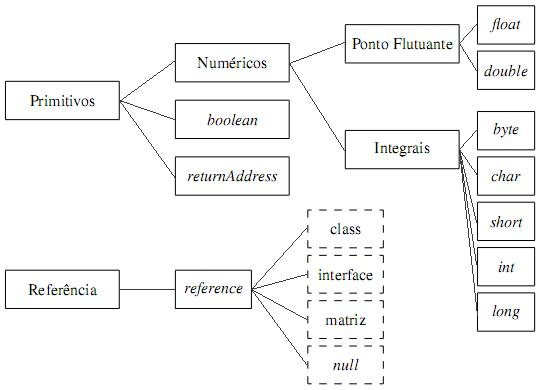
\includegraphics[width=0.8\textwidth]{imgs/java_data_types.jpg}
	\caption{Tipos de dados da m�quina virtual Java}	
	\label{fig:jvm-datatypes}
\end{figure}

%\begin{figure}[h]
% \def\captext{Caso de Uso Interface com o Usu�rio}
% \newlength{\ancho}
% \settowidth{\ancho}{Figura 3.1: \captext}
%     \centering
%     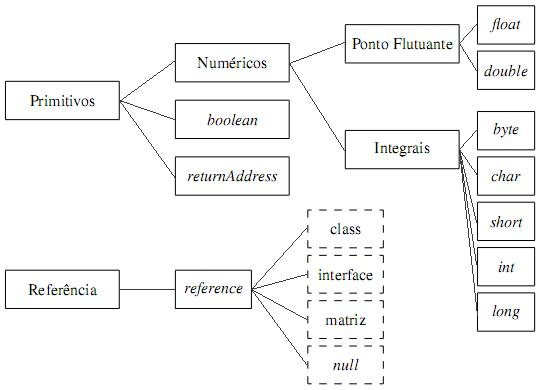
\includegraphics[width=0.90\textwidth]{imgs/java_data_types.jpg}
%     \parbox{\ancho}{\caption{\captext}
%     \makebox[\width]{Fonte: baseado em X.}}
%     \label{interface}
%\end{figure}

Todos os tipos primitivos da linguagem Java s�o tipos primitivos na JVM. Embora o tipo $boolean$
seja dito primitivo, o conjunto de instru��es tem um suporte limitado a ele. Quando um compilador traduz
c�digo Java para \textit{bytecodes}, ele utiliza $int$s e $byte$s para representar dados $boolean$.
Na m�quina virtual $false$ � representado pelo inteiro zero, e $true$ por qualquer inteiro diferente de zero.
Inteiros tamb�m s�o utilizados em opera��es envolvendo o tipo $boolean$. Matrizes de $boolean$ s�o representadas
como matrizes de $byte$.

Assim como na linguagem Java, os tipos primitivos da JVM possuem o mesmo intervalo de valores, independentemente
de plataforma operacional ou do \textit{hardware} sendo utilizado. Embora os intervalos de valores sejam
especificados, os tamanhos de cada tipo de dado n�o o s�o, ficando a crit�rio de quem implementa
a m�quina virtual.

A JVM trabalha com um tipo primitivo que n�o � disponibilizado ao programador da linguagem Java, o tipo
$returnAddress$. Este tipo � utilizado na linguagem, na implementa��o de cl�usulas $finally$.

O tipo refer�ncia da JVM � chamado de $reference$. Valores deste tipo podem ser: de classe (\textit{class type}), 
de interface (\textit{interface type}) e de matriz (\textit{array type}). Todos possuem como valores
refer�ncias para objetos criados dinamicamente. Um outro valor de $reference$ � $null$, o qual
indica que a vari�vel n�o referencia nenhum objeto.

Os intervalos dos tipos de dado da JVM s�o mostrados na tab.~\ref{tab:jvm-data-ranges}.

\begin{table}[h]
	\caption{Intervalo dos tipos de dados da m�quina virtual Java}
	\label{tab:jvm-data-ranges}
	
\begin{center}
\begin{tabular}{ll}\hline\hline
	\textbf{Tipo} & \textbf{Intervalo} \\
	$byte$ & inteiro de 8-bits com sinal ($-2^7$ at� $2^7 - 1$, inclusive) \\
$short$ & inteiro de 16-bits com sinal ($-2^{15}$ at� $2^{15} - 1$, inclusive) \\
$int$ & inteiro de 32-bits com sinal ($-2^{31}$ at� $2^{31} - 1$, inclusive) \\
$long$ & inteiro de 64-bits com sinal ($-2^{63}$ at� $2^{63} - 1$, inclusive) \\
$char$ & caractere Unicode sem sinal de 16-bits ($0$ at� $2^{16} - 1$, inclusive) \\
$float$ &	ponto flutuante com precis�o simples de 32-bits no padr�o IEEE 754 \\
$double$ & ponto flutuante com precis�o dupla de 64-bits no padr�o IEEE 754 \\
$returnAddress$ & endere�o de um \textit{opcode} dentro do mesmo m�todo \\
$reference$ & refer�ncia para um objeto na $heap$, ou $null$ \\
\hline\hline
\end{tabular}
\end{center}
\end{table}


\section{�reas de Mem�ria}

Na especifica��o da JVM s�o definidas v�rias �reas de mem�ria. Algumas destas s�o alocadas quando a m�quina
virtual � inicializada e desalocadas quando a JVM termina a sua execu��o.
Outras s�o alocadas juntamente na cria��o da \textit{thread}, e desalocadas com o t�rmino de sua execu��o.

% O registrador PC
A JVM suporta a execu��o de v�rias \textit{threads}, onde cada uma possui um registrador \textit{program counter} - PC \sigla{PC}{\textit{Program Counter} - Contador de programa}. Este registrador
cont�m o endere�o da instru��o no m�todo sendo executado no momento pela \textit{thread}, por�m, se o m�todo
for nativo, o conte�do do registrador � indefinido.

Veremos em mais detalhes, nas pr�ximas subse��es, as principais �reas de mem�ria da JVM.

\subsection{�rea de M�todos}

Dentro de uma inst�ncia da JVM, as informa��es sobre os tipos carregados ficam armazenados em um local na
mem�ria chamado de �rea de m�todos. Quando a m�quina virtual carrega algum tipo, um carregador de classes
(\textit{class loader}) localiza e carrega a classe, para que ent�o algumas informa��es sejam extra�das.
Estas informa��es extra�das s�o guardadas na �rea de m�todos, mas a forma em que s�o armazenadas fica a 
crit�rio da implementa��o.

Durante a execu��o da aplica��o, a JVM ir� fazer buscas nessas informa��es de tipos, e, por isso, essas
informa��es devem estar armazenadas de uma forma otimizada para que as buscas sejam r�pidas. 

Como esta �rea de mem�ria � compartilhada entre todas as \textit{threads} em execu��o pela JVM, o acesso �s 
estruturas de dados da �rea de m�todos deve ser projetado para ser \textit{thread-safe}. Se duas
\textit{threads} tentam utilizar uma classe que n�o est� carregada, ent�o a primeira que realizou a solicita��o
ter� a prioridade de carreg�-la, enquanto a outra espera.

O tamanho da �rea de mem�ria n�o precisa ser fixo. A m�quina virtual pode expandir e contrair a �rea de m�todos
da maneira que a aplica��o necessitar. Ainda com rela��o � mem�ria da �rea de m�todos, esta pode ser n�o
continua \cite{jvmspec}.

Durante a execu��o do programa, classes podem n�o ser mais referenciadas. Assim, as informa��es armazenadas
na �rea de m�todos podem ser liberadas por um \textit{garbage collector}, mantendo no m�nimo poss�vel o tamanho
ocupado.

Para cada tipo que a JVM carrega, uma tabela de s�mbolos (\textit{constant pool}) deve ser armazenada.
Esta tabela � um conjunto de constantes que s�o usados pelo tipo, incluindo literais e refer�ncias
simb�licas para tipos, campos e m�todos. As entradas nessa tabela s�o acessadas atrav�s de um �ndice, assim
como os elementos de uma matriz \cite{insidejvm}.

\subsection{Heap}

A \textit{heap} � a �rea de dados onde as inst�ncias de classes e as matrizes s�o alocadas.

Assim como a �rea de m�todos, a \textit{heap}: � compartilhada entre todas as \textit{threads} da JVM,
bem como � criada na inicializa��o da m�quina virtual, podendo ter um tamanho fixo ou ser expandida/contra�da 
sob demanda, n�o precisando a sua �rea de mem�ria ser continua.

Embora a JVM tenha uma instru��o para alocar mem�ria na \textit{heap} para um novo objeto, n�o h� uma instru��o
que libera a mem�ria alocada por este objeto. Fica sob responsabilidade da implementa��o da JVM a libera��o
da mem�ria ocupada por objetos que n�o s�o mais referenciados na aplica��o, sendo que, normalmente,
a m�quina virtual utiliza algum algoritmo de \textit{garbage collection} para a libera��o da mem�ria.

\subsection{Pilha da \textit{Thread}}

Em conjunto com a cria��o de uma \textit{thread} � criada uma pilha (JVM \textit{stack}), que cont�m
p�ginas (\textit{frames}). As p�ginas dessa pilha atuam de maneira similar aos registros de ativa��o de linguagens,
como por exemplo a linguagem C. A fun��o da p�gina � armazenar os par�metros, as vari�veis locais, a pilha 
de operandos e alguns dados pr�prios.

As vari�veis locais na p�gina est�o organizadas em uma matriz de palavras (\textit{words}), onde o primeiro
�ndice � zero. Palavra � a unidade b�sica de tamanho para os tipos de dados na JVM. Pela especifica��o
da JVM, uma palavra deve ter o tamanho necess�rio para armazenar um valor de tipo $byte$, $short$, $int$, $char$,
$float$, $returnAddress$, ou $reference$. Duas palavras devem comportar um $long$ ou $double$. O tamanho de uma
palavra geralmente � definido como sendo o tamanho de um ponteiro nativo na plataforma do hospedeiro.
Valores de tipo $byte$, $short$, e $char$ s�o convertidos para $int$ antes de serem colocadas nas vari�veis locais.
Valores de tipo $long$ e $double$ ocupam dois lugares consecutivos na matriz.

Assim como as vari�veis locais, a pilha de operandos na p�gina � uma matriz de palavras. Por�m, a pilha de 
operandos n�o � acessada atrav�s de �ndices, mas, atrav�s de opera��es de empilhar e desempilhar.

Alguns dados pr�prios na p�gina da pilha da JVM s�o utilizados para ajudar no acesso a dados que est�o na
tabela de s�mbolos, bem como para retornar o resultado do m�todo a quem o chamou, ou, em casos de t�rmino
por exce��o, guardar informa��es sobre a exce��o que ocorreu.

A m�quina virtual executa apenas duas opera��es na pilha: empilha e desempilha p�ginas. Quando um m�todo
� chamado, � criada e empilhada uma nova p�gina na pilha, e esta torna-se a p�gina atual.
Um m�todo pode terminar de forma normal, quando termina a sua computa��o, ou de forma repentina,
com o lan�amento de uma exce��o. De ambas maneiras, a m�quina virtual desempilha a p�gina do m�todo sendo
executado, e descarta-o. Ent�o, a p�gina do m�todo anterior, que est� no topo da pilha, passa a ser a p�gina atual.

Todos os dados na pilha da \textit{thread} s�o privados �quela \textit{thread}. Desta forma, o acesso a
vari�veis locais nos m�todos n�o precisa ser sincronizado, pois as vari�veis locais estar�o alocadas em
uma p�gina na pilha da \textit{thread} que chamou o m�todo.

Assim como a �rea de m�todos e a \textit{heap}, a �rea de mem�ria em que est� a pilha ou as p�ginas n�o
precisa ser continua.

\subsection{Pilha de M�todos Nativos}

Quando uma \textit{thread} chama um m�todo nativo, surge um novo mundo no qual as estruturas e as restri��es de
seguran�a da JVM n�o limitam mais o programador. Um m�todo nativo pode acessar as �reas de mem�ria discutidas
nas se��es anteriores (dependendo da interface de m�todos nativos que o implementador oferecer).
O programador poder� utilizar os registradores nativos do processador, alocar mem�ria diretamente do sistema
hospedeiro, etc.

Qualquer interface de m�todos nativos ir� usar algum tipo de pilha desses m�todos. Quando uma \textit{thread}
chama um m�todo, a m�quina virtual cria uma nova p�gina e empilha na pilha da JVM. Entretanto, quando uma
\textit{thread} chama um m�todo nativo, a pilha da JVM n�o � utilizada. Ao inv�s de empilhar uma nova p�gina,
a JVM ir� simplesmente ligar dinamicamente o m�dulo que oferece o m�todo, e cham�-lo.

Assim como em outras �reas de mem�ria, a mem�ria ocupada pelas pilhas de m�todos nativos n�o precisa ser
de um tamanho fixo, podendo expandir/contrair de acordo com a necessidade da aplica��o.

\section{Conjunto de Instru��es (\textit{opcodes})}
\label{sec:jvm-opcodes}

Cada instru��o da JVM consiste em um c�digo de opera��o de um byte (justificando o nome de \textit{bytecode}),
podendo necessitar de zero ou mais operandos. Quando operandos s�o necess�rios, ap�s o byte da instru��o seguem um ou mais bytes que podem representar o �ndice de uma vari�vel na matriz de vari�veis locais, um valor imediato ou uma refer�ncia � tabela de s�mbolos da classe \cite{jarismar2003}. Um pseudo-c�digo do la�o principal do
interpretador da JVM, ignorando exce��es, � mostrado na Figura~\ref{fig:loop-jvm-interpreter}.

\begin{figure}[h]
\progfig{
do \{\= \\
     \>busca um \textit{opcode}; \\
     \>if (\textit{opcode} exige operandos) busca operandos; \\
     \>executa a a��o do \textit{opcode} \\
\} while (tem mais a fazer); \\
}
	\caption{Pseudo-c�digo do la�o principal do interpretador da JVM}
	\label{fig:loop-jvm-interpreter}
\end{figure}
% TODO fonte jvmspec secao 3.11

Na maioria das instru��es com tipos, o tipo ao qual a instru��o se aplica � explicito no mnem�nico do
\textit{opcode} \sigla{opcode}{\textit{Operation Code} - C�digo de instru��o} pelas letras i, l, s, b, c, f, d, a, que correspondem, respectivamente, aos tipos $int$, $long$,
$short$, $byte$, $char$, $float$, $double$ e $reference$. Estas letras s�o utilizadas por toda a JVM,
e s�o chamadas de descritores de tipos.
Instru��es onde o tipo n�o � amb�guo n�o possuem
uma letra descrevendo o tipo no seu mnem�nico. Por exemplo, $arraylength$ sempre tem como operando um objeto
que � uma matriz. Algumas instru��es, como $goto$, possuem seus operandos sem tipo.

Nas subse��es a seguir veremos as principais categorias de instru��es que a JVM prov�.

\subsection{Instru��es de Vari�veis Locais e Pilha de Operandos}

Como a JVM � uma m�quina baseada em pilhas, quase todas as suas instru��es s�o relacionadas � pilha de operandos.
A maioria das instru��es empilham e desempilham valores, ou executam ambas opera��es.

As instru��es que transferem valores entre a pilha de operandos e as vari�veis locais s�o:

\begin{itemize}
	\item Carregam uma vari�vel local na pilha de operandos: \textit{iload}, \textit{iload\_<n>}, 
\textit{lload}, \textit{lload\_<n>}, \textit{fload}, \textit{fload\_<n>}, \textit{dload}, \textit{dload\_<n>}, \textit{aload}, \textit{aload\_<n>};

	\item Armazenam um valor da pilha de operandos em uma vari�vel local: \textit{istore}, \textit{istore\_<n>}, \textit{lstore},
\textit{lstore\_<n>}, \textit{fstore}, \textit{fstore\_<n>}, \textit{dstore}, \textit{dstore\_<n>}, \textit{astore}, \textit{astore\_<n>};

	\item Carregam uma constante na pilha de operandos: \textit{bipush}, \textit{sipush}, \textit{ldc}, \textit{ldc\_w}, \textit{ldc2\_w},
\textit{aconst\_null}, \textit{iconst\_m1}, \textit{iconst\_<i>}, \textit{lconst\_<l>}, \textit{fconst\_<f>}, \textit{dconst\_<d>};

	\item Ganha acesso a mais vari�veis locais usando um �ndice maior: \textit{wide}.
\end{itemize}

As instru��es acima que terminam com ``<n>'' indicam instru��es que oferecem operandos impl�citos, n�o sendo
necess�rio que o operando seja buscado ou armazenado. Por exemplo, \textit{iload\_0} empilha a vari�vel local
que est� no �ndice zero na pilha de operandos, o que � equivalente a instru��o \textit{iload 0}. Da mesma forma,
istore\_0 � equivalente a \textit{store 0}, e ambos armazenam na vari�vel local de �ndice zero o valor que est� 
no topo da pilha de operandos.

Existem tr�s maneiras de se empilhar constantes: o valor da constante estar impl�cito no \textit{opcode}
 (\textit{iconst\_1} empilha a constante um),
o valor da constante ser o operando do \textit{opcode} (\textit{iconst 1}), ou ent�o a constante vir da tabela de s�mbolos (\textit{ldc}). Como em alguns algoritmos � comum inicializarmos alguma vari�vel com o valor $-1$, os
projetistas da JVM inclu�ram o \textit{opcode} \textit{iconst\_m1}.

O �ndice para endere�ar vari�veis locais � de 8-bits, o que limita o n�mero m�ximo dessas para apenas 256.
A instru��o \textit{wide} pode estender o �ndice com outro de 8-bits, elevando o n�mero m�ximo de vari�veis
locais para 65536. Este \textit{opcode} precede � instru��o que deseja acessar alguma vari�vel local acima
do limite de 256.

\begin{table}[h]
	\caption{Instru��es que manipulam diretamente a pilha de operandos}
	\label{tab:stackops}

	\begin{center}
	\begin{tabular}{ll}\hline\hline
		\textbf{Instru��o} & \textbf{Descri��o} \\
\textit{nop} & n�o executa nada \\
\textit{pop} & desempilha a palavra do topo da pilha de operandos \\
\textit{pop2} & desempilha as duas palavras do topo da pilha de operandos \\
\textit{swap} & troca as duas palavras no topo da pilha \\
\textit{dup} & duplica o operando no topo da pilha \\
\textit{dup2} & duplica os dois operandos no topo da pilha \\
		\hline\hline
	\end{tabular}
	\end{center}
\end{table}

Embora a maioria das instru��es na JVM opere sobre um tipo, algumas instru��es manipulam a pilha de operandos
de forma independente de tipo. Estas instru��es s�o mostradas na tab.~\ref{tab:stackops}.

\subsection{Instru��es Aritm�ticas}

As instru��es aritm�ticas computam um resultado que � tipicamente uma fun��o de dois valores que est�o na pilha
de operandos, empilhando o resultado nesta. N�o h� suporte direto para opera��es aritm�ticas envolvendo valores
de tipos \textit{byte}, \textit{short}, \textit{char} e \textit{boolean}. Estes tipos s�o convertidos para
\textit{int} antes de serem colocados na pilha de operandos. As instru��es aritm�ticas s�o as seguintes:

\begin{itemize}
	\item Adi��o: Add: iadd, ladd, fadd, dadd;
	\item Subtra��o: isub, lsub, fsub, dsub;
	\item Multiplica��o: imul, lmul, fmul, dmul;
	\item Divis�o: idiv, ldiv, fdiv, ddiv;
	\item Resto: irem, lrem, frem, drem;
	\item Troca de sinal: ineg, lneg, fneg, dneg;
	\item Deslocamento: ishl, ishr, iushr, lshl, lshr, lushr;
	\item OR bit a bit: ior, lor;
	\item AND bit a bit: iand, land;
	\item XOR bit a bit: ixor, lxor;
	\item Incremento de vari�vel local: iinc;
	\item Compara��o: dcmpg, dcmpl, fcmpg, fcmpl, lcmp.
\end{itemize}

A JVM n�o indica a exist�ncia de \textit{overflow} durante opera��es com inteiros.
As �nicas opera��es com inteiros que podem lan�ar uma exce��o s�o as opera��es de divis�o entre inteiros
(\textit{idiv} e \textit{ldiv}) e as instru��es de resto inteiro (\textit{irem} e \textit{lrem}),
as quais lan�am uma exce��o \textit{ArithmeticException} se o divisor for zero.

\subsection{Instru��es de Convers�o de Tipos}

A JVM suporta as seguintes convers�es n�mericas:

\begin{itemize}
	\item \textit{int} para \textit{long} (\textit{i2l}), \textit{float} (\textit{i2f}) ou \textit{double} (\textit{i2d});
	\item \textit{long} para \textit{float} (\textit{l2f}) ou \textit{double} (\textit{l2d});
	\item \textit{float} para \textit{double} (\textit{f2d}).
\end{itemize}

Estas convers�es s�o utilizadas pois o programador explicitamente faz uma convers�o de tipo no seu programa,
ou ent�o ocorre implicitamente atrav�s da m�quina virtual, de modo a suprir a falta de algumas opera��es com
outros tipos n�mericos.

\subsection{Cria��o e Manipula��o de Objetos}

Embora tanto inst�ncias de classes como matrizes sejam objetos, a JVM as cria e manipula de formas distintas:

\begin{itemize}
	\item Cria uma nova inst�ncia de uma classe: \textit{new};	
	\item Cria uma nova matriz: \textit{newarray}, \textit{anewarray}, \textit{multianewarray};
	\item Acessa campos de classes (\textit{static fields}) e atributos de inst�ncias: \textit{getfield}, \textit{putfield}, \textit{getstatic}, \textit{putstatic};
	\item Carrega um item de uma matriz na pilha de operandos: \textit{baload}, \textit{caload}, \textit{saload}, \textit{iaload}, \textit{laload}, \textit{faload}, \textit{daload}, \textit{aaload};
	\item Armazenam um valor da pilha de operandos como um item de uma matriz: \textit{bastore}, \textit{castore}, \textit{sastore}, \textit{iastore}, \textit{lastore}, \textit{fastore}, \textit{dastore}, \textit{aastore};
	\item Coloca na pilha de operandos o tamanho da matriz: \textit{arraylength};
	\item Verifica propriedades de inst�ncias de classes e matrizes: \textit{instanceof}, \textit{checkcast}.
\end{itemize}

\subsection{Instru��es de Transfer�ncia de Controle}

As instru��es de transfer�ncia de controle, condicional ou incondicionalmente, fazem com que a JVM
pule para outras posi��es no m�todo, continuando com a sua execu��o. S�o elas:

\begin{itemize}
	\item Condicional: \textit{ifeq}, \textit{iflt}, \textit{ifle}, \textit{ifne}, \textit{ifgt}, \textit{ifge}, \textit{ifnull}, \textit{ifnonnull}, \textit{if\_icmpeq}, \textit{if\_icmpne}, \textit{if\_icmplt}, \textit{if\_icmpgt}, \textit{if\_icmple}, \textit{if\_icmpge}, \textit{if\_acmpeq}, \textit{if\_acmpne};
	\item Incondicional: \textit{goto}, \textit{goto\_w}, \textit{jsr}, \textit{jsr\_w}, \textit{ret};
	\item Para suportar a constru��o \textit{switch}: \textit{tableswitch}, \textit{lookupswitch}.
\end{itemize}

\subsection{Instru��es de Chamada e Retorno de M�todos}

As seguintes instru��es executam chamadas a m�todos:

\begin{itemize}
	\item \textit{invokevirtual} chama um m�todo em um objeto;
	\item \textit{invokeinterface} chama um m�todo que � implementado por uma interface, buscando a implementa��o correta do objeto a ser chamada em tempo de execu��o;
	\item \textit{invokespecial} chama um m�todo de um objeto que necessite de um tratamento especial, seja
um m�todo de inicializa��o de uma inst�ncia, um m�todo privado, ou um m�todo da classe pai (\textit{super});
	\item \textit{invokestatic} chama um m�todo est�tico em uma classe.
\end{itemize}

As instru��es que retornam os resultados nos m�todos s�o distinguidas pelo tipo de retorno. S�o elas:
\textit{ireturn} (usado em tipos \textit{boolean}, \textit{byte}, \textit{char}, \textit{short}, ou \textit{int}),
\textit{lreturn}, \textit{freturn}, \textit{dreturn} e \textit{areturn}. Para m�todos \textit{void}, que
n�o retornam nenhum resultado, m�todos inicializadores de inst�ncias, classes ou interfaces, � utilizada
a instru��o \textit{return}.

\subsection{Instru��es de Manipula��o de Exce��es}

Uma exce��o � lan�ada programaticamente usando a instru��o \textit{athrow}. Exce��es tamb�m podem ser lan�adas
por v�rias instru��es da JVM se uma condi��o anormal for detectada.

Blocos \textit{try \ldots catch} podem ter um bloco \textit{finally}, cujas instru��es s�o executadas
indiferentemente de haver uma exce��o ou n�o. A implementa��o de \textit{finally} pela JVM utiliza
as instru��es \textit{jsr}, \textit{jsr\_w}, e \textit{ret}.

\subsection{Instru��es para Sincroniza��o}

A sincroniza��o de sequ�ncias de instru��es � tipicamente utilizada nos m�todos com o modificador \textit{synchronized} da linguagem Java. A JVM oferece as instru��es \textit{monitorenter} e 
\textit{monitorexit} para suportar tal constru��o da linguagem.

\section{Execu��o}

A JVM inicia a execu��o de uma aplica��o chamando o m�todo \textit{main} de uma classe, cuja assinatura
� mostrada abaixo, onde \textit{args} s�o os par�metros passados para a aplica��o:

\progb{
	public static void main(String[] args)
}

A execu��o do m�todo \textit{main} ocorre na \textit{thread} principal, por�m, antes da execu��o,
a JVM realiza a liga��o e inicializa��o da classe. 

A liga��o envolve o processo de verifica��o, prepara��o e, opcionalmente, resolu��o.

O passo de verifica��o assegura que a representa��o carregada da classe a ser executada est� semanticamente 
correta. Se algum problema for detectado durante esta fase, um erro � lan�ado.

A prepara��o envolve a aloca��o de espa�o para as estruturas de dados que s�o utilizadas internamente pela 
m�quina virtual, como tabelas de m�todos.

Resolu��o � o processo de verificar as refer�ncias simb�licas para as outras classes e interfaces, carregando-as
e verificando se as refer�ncias est�o corretas.

A inicializa��o da classe consiste na execu��o dos inicializados est�ticos da classe, de acordo com a ordem no
programa (\textit{textual order}). Por�m, antes da inicializa��o da classe, sua classe pai deve ser inicializada,
assim como todas as outras classes que est�o acima na hierarquia de classes. No caso mais simples, a classe pai
ser� Object (\textit{java.lang.Object}).

Ap�s todos esses passos, o m�todo \textit{main} � executado.

\section{Especifica��o dos Arquivos \textit{.class}}
\label{sec:spec-class}

O arquivo \textit{.class} � um arquivo bin�rio, em um formato definido para que programas possam ser executados
na JVM, de forma independente de plataforma e da implementa��o da m�quina virtual. Cada arquivo
\textit{.class} cont�m a descri��o completa de uma, e somente uma, classe ou interface Java.

Os dados s�o armazenados sequencialmente no arquivo, sem espa�amento (\textit{padding}) ou alinhamento
(\textit{alignment}) entre eles. Esta falta de espa�amento refor�a o cuidado dos projetistas da JVM em manter
o \textit{bytecode} compacto.
Os dados dos itens das estruturas de dados que representam a classe/interface que ocuparem mais de um \textit{byte} s�o divididos e organizados na ordem \textit{big-endian}
\footnote{Neste formato, os bytes de maior ordem ficam nas primeiras posi��es, o caso contr�rio � chamado de
\textit{little-endian}.}.

O presente trabalho n�o ir� descrever a estrutura dos arquivos \textit{.class}, visto que um extenso estudo
sobre o tema pode ser encontrado em \citeonline{jarismar2003}.


% capitulo3.tex
\chapter{Implementa��o}

Neste trabalho foi implementado um compilador para uma linguagem funcional que tem \textit{bytecodes}
Java como o seu c�digo objeto. A linguagem funcional definida tem sintaxe similar a de Haskell,
sua ordem de avalia��o � estrita,
� estaticamente tipada, possui infer�ncia de tipos e n�o possui suporte � sobrecarga (\textit{overload}).
O compilador possui no seu \textit{frontend} um analisador sint�tico e um inferidor de tipos, e seu
\textit{backend} gera os \textit{bytecodes} Java.

As se��es seguintes demonstram os recursos do compilador desenvolvido, bem como alguns aspectos de sua
implementa��o e utiliza��o.

\section{Analisador Sint�tico}

O analisador sint�tico � uma parte de um compilador ou interpretador, cuja fun��o � verificar se o texto de
entrada (c�digo fonte) est� de acordo com a especifica��o l�xica e sint�tica da gram�tica especificada. 
Os analisadores l�xicos e sint�ticos podem ser implementados ou gerados semi-automaticamente por uma ferramenta 
que tem como entrada uma gram�tica escrita em BNF \sigla{BNF}{Backus Naur \textit{Form} - Forma de Backus Naur}.

Neste trabalho, o analisador sint�tico foi programado sem o aux�lio de uma ferramenta, utilizando 
uma biblioteca de combinadores mon�dicos em Haskell chamada de Parsec, o qual � visto em maiores 
detalhes na pr�xima se��o.

\subsection{Parsec}

Parsec � uma biblioteca de combinadores mon�dicos em Haskell. Combinadores s�o fun��es de ordem superior 
que s�o utilizadas de forma infixa, e ditas mon�dicas porque lidam com m�nadas.

Ao contr�rio de ferramentas que geram analisadores sint�ticos, como o cl�ssico Yacc \sigla{Yacc}{\textit{Yet Another Compiler Compiler} - Ainda outro compilador de compiladores} \cite{yacc}, que oferecem
um conjunto fixo de combinadores para definir gram�ticas, os combinadores mon�dicos s�o manipulados como
valores de primeira classe\footnote{Valor de primeira classe (\textit{first-class value} ou tamb�m as
variantes \textit{first-class object}, \textit{first-class citizen} e \textit{first-class object}) � uma 
entidade que pode ser usada sem restri��es em programas (sem restri��es quando comparado com outros objetos
na mesma linguagem). O termo foi cunhado por Christopher Strachey na d�cada de 1960.} e podem ser
combinados de forma a definirem analisadores mais espec�ficos \cite{meijer2001a}.
Outra vantagem � que o programador utiliza apenas uma linguagem, evitando a integra��o de diferentes linguagens
e ferramentas \cite{hughes2000}.

Uma restri��o do Parsec, e da maioria dos analisadores baseados em combinadores, � que n�o h� uma maneira de
lidar com recurs�o � esquerda. Caso uma produ��o seja recursiva � esquerda, o analisador entrar� em um \textit{loop} infinito.
Uma solu��o � a reescrita da gram�tica, uma vez que toda gram�tica recursiva � esquerda pode ser reescrita como recursiva � direita \cite{aho86}. Outra solu��o � a utiliza��o de um combinador $chainl$ \cite{fokker95}, que
implementa o padr�o de reescrita da gram�tica.

O Parsec j� vem incluso na instala��o do Glasgow Haskell Compiler - GHC \sigla{GHC}{Glasgow Haskell \textit{Compiler} - Compilador Haskell de Glasgow}, e pode ser importado atrav�s
do m�dulo \textit{Text.ParserCombinators.Parsec}.

Para construir um exemplo de uso do Parsec, vamos definir uma simples gram�tica para blocos de linguagens 
de programa��o:

\progb{
	<sentenca> ::= letras ou n�meros \\
	<bloco> = { [ <sentenca> ; ]+ }
}

Um bloco cont�m uma lista de senten�as, e este � o resultado da avalia��o da fun��o $bloco$ do exemplo abaixo:

\progb{
import Text.ParserCombinators.Parsec\\
\\
separador \== char ';' \\
sentenca \>= many alphaNum\\
bloco \>= do  \=char '\{'; \\
            \>\>sentencas <- sentenca `endBy1` separador \\
            \>\>char '\}'; \\
            \>\>return sentencas
}

As fun��es \textit{many}, \textit{alphaNum}, \textit{endBy1} e \textit{char} s�o combinadores mon�dicos
fornecidos pelo Parsec.
Para testar o analisador, podemos utilizar a fun��o $parseTest$:

\progb{
*Main> parseTest bloco "\{sentenca1;sentenca2;\}" \\
$[$"sentenca1","sentenca2"$]$
}

Vamos testar o caso onde uma senten�a fica sem o ponto e v�rgula no seu final:

\progb{
*Main> parseTest body "\{sentenca1\}"\\
parse error at (line 1, column 11):\\
unexpected "\}"\\
expecting letter or digit or ";"
}

Como pode-se ver no exemplo acima, a biblioteca n�o apenas informa em qual linha do texto de entrada o 
erro ocorreu, como tamb�m lista as possibilidades de produ��o (como o conjunto PRIMEIROS de um n�o-terminal).
Uma das vantagens � que podemos associar uma mensagem de erro com os combinadores utilizando-se o combinador
de erro \textit{<?>}. Reescrevendo o exemplo anterior com mensagens de erro personalizadas:

\progb{
separador \== char ';' <?> ``separador de sentenca'' \\
sentenca \>= many (alphaNum <?> ``sentenca'')\\
bloco \>= do  \=char '\{'; \\
            \>\>sentencas <- sentenca `endBy1` separador \\
            \>\>char '\}'; \\
            \>\>return sentencas
}

Testando esta nova defini��o obtemos:

\progb{
*Main> parseTest body "\{sentenca1\}"\\
parse error at (line 1, column 11):\\
unexpected "\}"\\
expecting sentenca or separador de sentenca
}

Para conhecer outros combinadores e obter a documenta��o dos utilizados no exemplo desta se��o consulte 
a documenta��o do Parsec \cite{parsec-doc}.

\subsection{C�digo Intermedi�rio}

De acordo com o texto de entrada, o analisador sint�tico armazena em suas estruturas de dados uma representa��o
intermedi�ria, chamada de c�digo intermedi�rio. Nesta subse��o veremos as principais estruturas utilizadas,
bem como os seus significados.

A representa��o adotada foi inspirada nos tipos alg�bricos usados por Mark P. Jones \cite{Mark99}
para descrever informalmente o sistema de infer�ncia de tipos da linguagem Haskell.

\subsubsection{Identificadores}

Os identificadores da linguagem s�o representados pelo tipo \textit{Id}, que armazena uma \textit{string}
com o nome do identificador e tamb�m um inteiro representando o n�vel da sua declara��o. Um n�vel de valor
zero indica um identificador declarado no escopo global, e maiores que zero, indicam vari�veis declaradas
atrav�s do comando \textit{let}.

\progb{
	data Id = Id String Int
}

\subsubsection{Tipos}

Os tipos s�o representados atrav�s do tipo alg�brico \textit{Type}. As express�es de tipos podem ser:
vari�veis de tipo (\textit{TVar}), construtores de tipos (\textit{TCon}), aplica��es de um tipo para outro
(\textit{TAp}) e tipos polim�rficos (tamb�m chamados de vari�veis de tipo quantificadas).

\progb{
data Type \== TVar Tyvar \\
			\>$|$ TCon Tycon \\
			\>$|$ TAp Type Type \\
			\>$|$ TGen Int \\
\\
data Tyvar = Tyvar String [Int] \\
data Tycon = Tycon Id
}

Apresentamos abaixo alguns exemplos de como representar tipos primitivos da linguagem utilizando os construtores
de tipos:

\progb{
	tChar  \== TCon (Tycon (Tycon (Id "Char" 0))) \\
	tArrow \>= TCon (Tycon (Tycon (Id "(->)" 0))) \\
	tList	 \>= TCon (Tycon (Tycon (Id "[]" 0)))
}

Uma fun��o auxiliar \textit{fn} � utilizada para facilitar a cria��o de tipos para fun��es:

\progb{
infixr 4 `fn` \\
fn :: Type -> Type -> Type \\
a `fn` b = TAp (TAp tArrow a) b
}

\subsubsection{Substitui��es}

As substitui��es t�m um papel importante na infer�ncia de tipos, pois mapeiam vari�veis de tipo para tipos.

\progb{
	type Subst  = [(Tyvar, Type)]
}

Como as substitui��es podem ser aplicadas a tipos ou a qualquer estrutura que os contenha, ent�o a fun��o
de aplica��o (\textit{apply}) deve ser sobrecarregada para diferentes tipos. Para isso implementamos uma
classe:

\progb{
cla\=ss Subs t where \\
  \>apply :: Subst -> t -> t \\
  \>tv    :: t -> [Tyvar]
}

A fun��o \textit{tv} retorna um conjunto de vari�veis de tipo que est�o contidas em seu argumento,
ordenadas por ordem de ocorr�ncia.

\subsubsection{Esquemas de Tipo (\textit{Type Scheme})}

\textit{Type schemes} s�o utilizados na representa��o de tipos polim�rficos, tamb�m chamados
de tipos quantificados.

\progb{
data Scheme = Forall Type
}

\subsubsection{Suposi��es de Tipo}
\label{sec:assump}

Suposi��es sobre o tipo de uma vari�vel s�o representadas por valores de \textit{Assump}. 
Uma dupla com o tipo de defini��o (\textit{Kind\_of\_defining\_occurrence}) e com o esquema de tipo
(\textit{Scheme}) � associado a um identificador:

\progb{
data Assump = Id :>: (Kind\_of\_defining\_occurrence, Scheme) \\
data Kind\_of\_defining\_occurrence = CW $|$ LB
}

O tipo de defini��o (\textit{Kind\_of\_defining\_occurrence}) indica se a vari�vel � ligada a uma
$\lambda{}$-abstra��o.

\subsubsection{Literais}

Valores literais s�o representados por \textit{Literal}:

\progb{
data Literal \== LitInt   Integer \\
			 \>$|$ LitChar  Char \\
			 \>$|$ LitStr   String \\
			 \>$|$ LitFloat Double
}

\subsubsection{Padr�es}

Padr�es (do ingl�s \textit{patterns}) s�o utilizados para inspecionar e desconstruir valores de tipos
alg�bricos. Os padr�es ser�o representados atrav�s de inst�ncias do tipo \textit{Pat}:

\progb{
data Pat \== PVar Id \\
			\>$|$ PLit Literal \\
			\>$|$ PCon Assump [Pat] \\
			\>$|$ PWildcard
}

O construtor \textit{PVar} representa vari�veis que est�o no padr�o, da mesma forma literais por \textit{PLit},
constru��es de padr�es por \textit{PCon}, e um padr�o coringa por \textit{PWildcard} (representado em programas
como ``\_'').

A seguinte fun��o retorna o primeiro elemento de uma lista: 

\progb{
head :: [a] -> a \\
head (x:\_) = x
}

Para fazer isto, a lista � desconstru�da atrav�s
do construtor de listas ``:'' em dois padr�es: um padr�o para a cabe�a da lista ($x$) e outro que ignora
o resto da lista. O retorno da fun��o � o valor da vari�vel $x$, que � associada ao padr�o.

O c�digo intermedi�rio gerado pelo analisador sint�tico para o padr�o da fun��o \textit{head} �:

\progb{
	PCon (\textit{Assump para ``:''}) [PVar (Id "x"~0),PWildcard]
}

\subsubsection{Express�es}

As express�es s�o representadas por inst�ncias de \textit{Expr}:

\progb{
data Expr \== Var Id \\
		  \>$|$ Lit Literal \\
		  \>$|$ Const Assump \\
		  \>$|$ Ap Expr Expr \\
		  \>$|$ Let BindGroup Expr
}

Vari�veis e literais s�o representados, respectivamente, por \textit{Var} e \textit{Lit}.
O construtor \textit{Const} � utilizado para constantes com nomes, como, por exemplo, construtores de tipos.
A aplica��o de fun��es e a express�o \textit{let} s�o representadas, respectivamente, por \textit{Ap} e 
\textit{Let}.

\subsubsection{Alternativas}

Para explicar alternativas, vamos analisar o seguinte exemplo:

\progb{
	len :: [a] -> Int \\
	len [] = 0 \\
	len (x:xs) = 1 + len xs
}

Neste exemplo, se diz que a fun��o \textit{len} possui duas alternativas: a primeira retorna zero se a
lista passada � vazia, e a segunda retorna um somado ao tamanho da lista $xs$.

As alternativas para as fun��es s�o representadas atrav�s do tipo \textit{Alt}. 

\progb{
type Alt = ([Pat], Expr)
}

Este tipo � uma tupla,
cujo primeiro componente � uma lista de padr�es para cada um dos argumentos da fun��o, e o segundo
componente � a express�o associada �quela alternativa.

\subsubsection{\textit{Binding Groups}}

Os \textit{binding groups} s�o utilizados para agrupar todas as alternativas para um identificador,
e podem ser expl�citos e impl�citos:

\begin{itemize}
	\item Expl�citos: este tipo de \textit{binding group} representa fun��es em que o programador fez 
uma declara��o expl�cita do seu tipo. Estes tipos ser�o verificados na fase de infer�ncia.

	\progb{
	type Expl = (Id, Scheme, [Alt])
	}

	\item Impl�citos: representam fun��es sem tipo expl�cito, que ter�o seus tipos inferidos durante o processo
de infer�ncia.

	\progb{
	type Impl = (Id, [Alt])
	}

\end{itemize}

Desta forma, um programa em Haskell pode ser representado por um tipo \textit{BindGroup}, que armazena
a lista de \textit{binding groups} expl�citos e impl�citos:

\progb{
type BindGroup = ([Expl], [Impl])
}

\subsubsection{Exemplos de sa�das}

Vejamos dois exemplos de programas escritos na sintaxe da linguagem definida neste trabalho,
analisando tamb�m a sa�da gerada pelo analisador sint�tico.

Neste primeiro exemplo, vamos declarar um tipo de dado de enumera��o para algumas cores:

\begin{figure}
	\progfig{
	\{ data Cores = Azul $|$ Verde $|$ Vermelho; \}
	}
	\caption{Exemplo de tipo de dado de enumera��o para cores}
	\label{fig:enum-cores}
\end{figure}

Uma vez que o analisador sint�tico ainda n�o fornece suporte a \textit{layouts}, o programa deve ser
declarado em um bloco entre chaves e cada declara��o do programa
deve ser terminada em ponto e v�rgula, sendo que a �ltima opcional.

A sa�da do analisador sint�tico para o exemplo da Fig.~\ref{fig:enum-cores} � mostrada na
 Fig.~\ref{fig:saida-enum-cores}.

\begin{figure}[ht]
	\progfig{
	(\=[], $--$ N�o h� nenhum \textit{binding group} expl�cito (\textit{Expl}) \\
	 \>[\={} $--$ Lista de \textit{binding groups} impl�citos (\textit{Impl}) \\
	  \>\>(I\=d "Azul"{} 0, $--$ Identificador ``Azul'' � definido em escopo global \\
	  	\>\>\>[ \={}$--$ Lista de alternativas (\textit{Alt}) \\
	  		\>\>\>\>(\=[], $--$ Nenhum padr�o (\textit{Pat}) \\
	  		 \>\>\>\>\>$--$ Para um construtor de tipo, utilizamos o construtor \textit{Const} de \textit{Expr} \\
	  		 \>\>\>\>\>$--$ :>: � um construtor de suposi��es, assim, para todo ``Azul'' temos \\
	  		 \>\>\>\>\>$--$  a suposi��o de tipo que ``Azul'' � do tipo ``Cor'' \\
	  		 \>\>\>\>\>Const (Id "Azul"{} 0 :>: (CW,Forall (TCon (Tycon (Id "Cor"{} 0))))) \\
	  		\>\>\>\>) \\
	  	\>\>\>] \\
	  \>\>), $--$ A explica��o acima vale para os demais construtores de Cor \\
	  \>\>(Id \="Verde"{} 0, \\
	  \>\>\>[([],Const (Id "Verde"{} 0 :>: (CW,Forall (TCon (Tycon (Id "Cor"{} 0))))))]), \\
	  \>\>(Id "Vermelho"{} 0, \\
	  \>\>\>[([],C\=onst (Id "Vermelho"{} 0 :>: \\
	  \>\>\>\>(CW,Forall (TCon (Tycon (Id "Cor"{} 0))))))]) \\
	 \>]) \\
	}
	
	\caption{Sa�da do analisador sint�tico para o exemplo da Fig.~\ref{fig:enum-cores}}
	\label{fig:saida-enum-cores}
\end{figure}

Neste segundo exemplo, mostrado na Fig.~\ref{fig:func-len}, vamos definir uma fun��o polim�rfica que calcula o tamanho de uma lista.

\begin{figure}[ht]
	\progfig{
	\{               \= \\
	\>len $[]$ = 0 \\
	\>len (x:xs) = 1 + len xs \\
	\}
	}
	
	\caption{Implementa��o da fun��o \textit{len}}
	\label{fig:func-len}
\end{figure}

Como n�o especificamos o tipo da fun��o \textit{len}, a lista de \textit{binding groups} expl�citos,
assim como no exemplo anterior, � vazia. Por este motivo, vamos omitir algumas informa��es para
simplificar a sa�da, mostrada na Fig.~\ref{fig:saida-func-len}.

\begin{figure}[ht]
	\progfig{
	[ \={} $--$ Lista de \textit{Impl}\\
		\>(I\=d "len"{} 0, \\
			\>\>[\={}  $--$ Lista de \textit{Alt}\\
			 \>\>\>(\=[PCon \{- Suposi��o de tipo para [] -\} []], $--$ Padr�o \\
			  \>\>\>\>Lit (LitInt 0) $--$ Express�o \\
			 \>\>\>), \\
			 \>\>\>( $--$ Padr�o \\
			 	\>\>\>\>[\=PCon \{- Suposi��o de tipo para (:) -\} [\=PVar (Id "x"{} 0),\\
			 	\>\>\>\>\>\>PVar (Id "xs"{} 0)]], \\
			 	 \>\>\>\>\>$--$ Express�o \\
			 	 \>\>\>\>\>$--$ Podemos notar que ``1 + len xs'' � o mesmo que a aplica��o \\
			 	 \>\>\>\>\>$--$ da fun��o (+1) com a fun��o (len xs) \\
			   \>\>\>\>\>Ap \=(Ap (Var (Id "+"{} 0)) (Lit (LitInt 1))) \\
			   \>\>\>\>\>\>(Ap (Var (Id "len"{} 0)) (Var (Id "xs" 0))) \\
			 \>\>\>) \\
			\>\>]  $--$ Final da lista de \textit{Alt}\\
		\>) \\
	]
	}

	\caption{Exemplo de sa�da do analisador sint�tico para a fun��o \textit{len}}
	\label{fig:saida-func-len}
\end{figure}


\section{Inferidor de Tipos}

O inferidor de tipos possui como principal estrutura de dados o tipo alg�brico \textit{Assump},
que j� foi descrito na se��o \ref{sec:assump}. Um contexto de tipos � uma lista de suposi��es de tipo,
representado pelo tipo sin�nimo \textit{TypCtx}:

\progb{
type TypCtx  = $[$Assump$]$
}

No come�o do processo de infer�ncia de tipos � passado um contexto de tipo inicial. Algumas das suposi��es
que comp�em o contexto inicial s�o mostradas abaixo:

\progb{
		  "+"{} :>: (CW, Forall (tInt `fn` tInt `fn` tInt)) \\
		  "$-$"{} :>: (CW, Forall (tInt `fn` tInt `fn` tInt)) \\
		  "*"{} :>: (CW, Forall (tInt `fn` tInt `fn` tInt)) \\
		  "/"{} :>: (CW, Forall (tInt `fn` tInt `fn` tFloat)) \\
		  "\&\&"{} :>: (CW, Forall (tBool `fn` tBool `fn` tBool)) \\
		  "$||$"{} :>: (CW, Forall (tBool `fn` tBool `fn` tBool)) \\
		  "not"{} :>: (CW, Forall ((tBool `fn` tBool))) \\
		  "True"{} :>: (CW, Forall tBool) \\
		  "False"{} :>: (CW, Forall tBool) \\
		  "[]"{} :>: (CW, (Forall (TAp tList (TGen 0)))) \\
		  ":"{}  :>: (CW, (Forall \=(TGen 0 `fn` \\
		  					\>TAp tList (TGen 0) `fn` TAp tList (TGen 0))))
}

Baseado nesse contexto inicial, o tipo de cada declara��o de fun��o � inferido por um algoritmo similar
ao algoritmo W, mostrado na Fig.~\ref{fig:algoritmoW}. 

Em uma segunda etapa, os tipos inferidos para as declara��es s�o unificados com os tipos requeridos.
O tipo requerido � o tipo que foi inferido no momento da aplica��o de uma fun��o.
Para que n�o exista a necessidade de uma ordena��o topol�gica baseada na ordem de aplica��o de fun��es,
foi utilizado para a unifica��o dos tipos, inferidos e requeridos, o algoritmo proposto por \citeonline{Vas03}.

\section{Sa�da do Compilador (\textit{backend})}

Tendo como entrada o c�digo intermedi�rio e os tipos inferidos do programa, o objetivo da �ltima parte
do compilador � gerar \textit{bytecodes} Java. Nas subse��es a seguir, veremos como s�o gerados os 
arquivos \textit{.class} e quais as tradu��es que ocorrem para se obter um c�digo orientado a objeto
a partir de um c�digo funcional.

\subsection{Jasmin}

Um dos objetivos deste trabalho � gerar \textit{bytecodes} Java para programas funcionais. Estes arquivos
\textit{.class}, como j� foi visto na se��o \ref{sec:spec-class}, s�o arquivos bin�rios.
Geralmente os compiladores de linguagens nativas, por exemplo de C, geram um arquivo texto que cont�m 
a representa��o do programa em uma linguagem de montagem (\textit{assembly}). Este arquivo � posteriormente
compilado por um montador para um formato bin�rio. Infelizmente, n�o h� uma linguagem de montagem e um
respectivo montador no \textit{kit} de desenvolvimento Java (Java Development Kit - JDK).
\sigla{JDK}{Java \textit{Development Kit} - Kit de desenvolvimento Java}

O padr�o \textit{de facto} de uma linguagem de montagem Java � o Jasmin \cite{jasmin}. Este montador recebe 
na sua entrada
um arquivo ASCII com descri��es das classes Java, em um formato simples e utilizando os mesmos nomes de 
\textit{opcodes} da JVM. O montador Jasmin ent�o converte estas descri��es para o formato bin�rio dos arquivos
\textit{.class}, que ent�o podem ser carregados normalmente pela JVM.

\sigla{JAR}{Java \textit{ARchive} - Arquivo Java}

O montador Jasmin � distribu�do atrav�s de um pacote Java (Java \textit{ARchive} - JAR), e o funcionamento
de como gerar os arquivos \textit{.class} � mostrado abaixo:

\progb{
	\$ java -jar jasmin.jar arquivo1.j arquivo2.j \ldots
}

\subsubsection{Formato do Arquivo Jasmin}

O formato do arquivo de montagem do Jasmin � mostrado abaixo:

\progb{
<arq\=uivo\_jasmin> \{ \\
    \><cabecalho> \\
    \>[<atributos>]* \\
    \>[<metodos>]* \\
\}
}

Apenas uma classe Java pode ser especificada por arquivo de montagem. Desta forma, informa��es sobre
a classe ficam na parte de cabe�alho, seguidas, opcionalmente, pelos atributos e m�todos da classe.

\progb{
	.class public NomeDaClasse \\
	.super java/lang/Object \\
	.implements nome/qualificado/da/Interface 
}

O c�digo de montagem acima � equivalente a seguinte classe Java:

\progb{
	public \=class NomeDaClasse \\
			   \>extends java.lang.Object  \\
			   \>implements nome.qualificado.da.Interface \{\}
}

Como podemos observar, a classe ``NomeDaClasse'' estende a classe \textit{Object} do pacote \textit{java.lang}
e implementa a interface declarada por \textit{nome.qualificado.da.Interface}.
Para declararmos um atributo inteiro, p�blico e com nome ``nomeDoAtributo'', usamos a seguinte linha:

\progb{
	.field public nomeDoAtributo I
}

A especifica��o dos tipos segue o padr�o dos descritores de tipos (vistos na se��o \ref{sec:jvm-opcodes}).

Resta-nos saber agora como descrever m�todos utilizando a linguagem Jasmin. Um exemplo que declara um m�todo
chamado ``umaString'', sem par�metros, p�blico, e que retorna uma \textit{string}, � mostrado abaixo:

\progb{
	.m\=ethod public umaString()Ljava/lang/String; \\
		\>ldc ``isto eh uma string'' \\
		\>areturn \\
	.end method
}

A partir do exposto at� agora, podemos escrever o cl�ssico exemplo de ``Al� mundo!'' em Jasmin:

\progb{
.class public Hello \\
.super java/lang/Object \\
\\
.m\=ethod public static main([Ljava/lang/String;)V \\
	\>.limit stack 2\\
		\\
	\>getstatic java/lang/System/out Ljava/io/PrintStream;\\
		\\
	\>ldc "Al� Mundo!"\\
		\\
	\>invokevirtual java/io/PrintStream/println(Ljava/lang/String;)V\\
		\\
	\>return\\
.end method\
}

Com a primeira linha dentro do m�todo, especificamos o limite de valores que podem ser empilhados na pilha
de operandos aritm�ticos. No exemplo acima, a pilha tem tamanho de duas posi��es e, como podemos notar, apenas 
as instru��es do montador come�am
com um ponto. As instru��es da JVM n�o s�o prefixadas por este. A instru��o \textit{getstatic} pega um
campo est�tico da classe do primeiro par�metro. Assim, no exemplo, se esta fazendo uma refer�ncia para
\textit{java.lang.System.out}, cujo tipo � \textit{java.io.PrintStream}.
Logo ap�s, a instru��o \textit{ldc} empilha um elemento que est� na tabela de s�mbolos (\textit{constant pool}),
no caso do exemplo, a \textit{string} ``Al� Mundo!''. Ap�s a prepara��o para a chamada do m�todo que ir�
imprimir na sa�da padr�o do processo Java, � executado o m�todo \textit{println} atrav�s da instru��o
\textit{invokevirtual}. No final do exemplo, temos a instru��o \textit{return}, fazendo com que a m�quina
virtual restabele�a o controle para o m�todo que efetuou a chamada. 

O resultado da execu��o, ap�s a montagem, do exemplo � a frase ``Al� Mundo!'' na tela.

Para maiores informa��es e detalhes de cada uma das declara��es poss�veis, basta consultar a documenta��o
do Jasmin \cite{jasmin}.

\subsection{Tradu��es}

A linguagem funcional definida neste trabalho possui dois tipos de declara��es: tipos de dados alg�bricos 
e fun��es.
� com base nestes que iremos definir as tradu��es do paradigma funcional para o orientado a objeto da JVM.
Embora o c�digo seja gerado na linguagem de montagem Jasmin, para facilitar a leitura, os exemplos
ser�o apresentados na linguagem Java.

Primeiramente, os tipos de dados alg�bricos, como j� vimos na se��o \ref{sec:tipos-algebricos}, s�o divididos
em: enumera��o, compostos, recursivos e polim�rficos. A tradu��o do tipo de dado alg�brico de enumera��o pode ser
feito atrav�s de um novo tipo de dado na vers�o 5 da linguagem Java, o tipo enumerado (\textit{enum type})
\cite{java-enum}, ou atrav�s do padr�o \textit{Typesafe Enum} \cite{bloch2008}, este compat�vel com vers�es
anteriores da JVM. 

Entretanto, este trabalho optou pela tradu��o desses tipos alg�bricos de uma maneira uniforme, de forma que
cada construtor do tipo alg�brico seja uma subclasse de uma classe abstrata que leva o nome do tipo.
A tradu��o para a linguagem Java do exemplo de tipo alg�brico de enumera��o da Fig.~\ref{fig:enum-cores} �
mostrada abaixo:

\progb{
	public abstract class Cores \{\} \\
	public Azul extends Cores \{\} \\
	public Verde extends Cores \{\} \\
	public Vermelho extends Cores \{\}
}

Diferentemente do tipo alg�brico de enumera��o, os demais tipos possuem construtores com par�metros.
Embora sejam tipos de dados, se passarmos apenas alguns par�metros para um construtor, estaremos fazendo
uma aplica��o parcial (currifica��o) sobre o tipo de dado. Por exemplo:

\progb{
\{ \\
	data Animal = Gato String Int \\
\}
}

O tipo do construtor \textit{Gato} � \textit{String} -> \textit{Int} -> \textit{Gato}, logo, s� teremos uma 
inst�ncia de \textit{Gato} se passarmos uma \textit{string} e um inteiro.
Como fun��es e tipos alg�bricos podem sofrer aplica��es parciais, podemos pensar em uma maneira uniforme 
de represent�-los. 

A representa��o escolhida � o uso de \textit{closures}, que consiste em um par de ponteiros,
um para o c�digo da fun��o e outro para o registro de ativa��o \cite{jmitchell2003}. Quando o \textit{closure}
vai ser executado � feito um salto para o endere�o do c�digo da fun��o. Em Java, isto ser� feito atrav�s
da chamada a um m�todo.

O presente trabalho definiu uma classe gen�rica e abstrata, chamada de \textit{Fun}, a qual possui 
um m�todo abstrato \textit{apply} que mapeia elementos de um tipo para outro. Esta classe representa a
id�ia do \textit{closure}, e o m�todo \textit{apply} a da execu��o do \textit{closure}.
A implementa��o da classe \textit{Fun} � mostrada abaixo:

\progb{
pu\=blic abstract class Fun<A, B> \{ \\
	\>public abstract B apply(A x); \\
\}
}

Isso significa que em tempo de compila��o as vari�veis de tipo \textit{A} e \textit{B} ser�o substitu�das 
pelos tipos especificados, garantindo que o programa esteja protegido pelo sistema de tipos contra erros 
de tipo.

Com base nisso, implementamos a tradu��o dos outros tipos alg�bricos como mostrado no exemplo abaixo, utilizando
como exemplo o tipo \textit{Animal}:

\progb{
public abstract class Animal \{\} \\
pu\=blic class Gato extends Animal \{ \\
	\>public String f1; \\
	\>public Integer f2; \\
	\>pu\=blic Gato(String f1, Integer f2) \{ \\
		\>\>this.f1 = f1; \\
		\>\>this.f2 = f2; \\
	\>\} \\
\} \\
public class GatoF1 extends Fun<String, GatoF1F2> \{ \\
	\>public GatoF1F2 apply(String x) \{ \\
		\>\>return new GatoF1F2(x); \\
	\>\} \\
\} \\
public class GatoF1F2 extends Fun<Integer, Gato> \{ \\
	\>public String f1; \\
	\>public GatoF1F2(String f1) \{ \\
		\>\>this.f1 = f1; \\
	\>\} \\
	\>public Gato apply(Integer x) \{ \\
		\>\>return new Gato(this.f1, x); \\
	\>\} \\
\}
}

O tipo alg�brico \textit{Animal} � traduzido em uma classe abstrata, pois n�o pode ser instanciada.
Cada um dos construtores de \textit{Animal} s�o subclasses deste. Se um construtor possui $n$ par�metros
ent�o ser�o geradas $n+1$ classes intermedi�rias. Cada uma delas recebe o valor de um par�metro, e retorna
a inst�ncia da pr�xima classe, que recebe o pr�ximo par�metro e retorna outra classe, etc. A classe que
receber o �ltimo par�metro retorna uma inst�ncia da que possui o nome do construtor.

Como o construtor de tipo \textit{Gato} possui dois par�metros, ser�o necess�rias tr�s classes: \textit{GatoF1}
que recebe em \textit{apply} o primeiro par�metro (\textit{String}) e retorna uma inst�ncia de \textit{GatoF1F2},
\textit{GatoF1F2} que recebe o segundo par�metro do construtor (\textit{Integer}), e \textit{Gato}, cuja inst�ncia � retornada por \textit{GatoF1F2} em seu m�todo \textit{apply}.

Uma vez que j� definimos uma maneira de se traduzir tipos alg�bricos, e tamb�m uma classe abstrata
\textit{Fun} que for�a suas subclasses a implementarem o m�todo \textit{apply}, podemos utilizar esta mesma
estrutura para implementar de uma maneira uniforme a tradu��o de fun��es.

Vamos utilizar como exemplo a fun��o \textit{map}, que atrav�s de uma fun��o, mapeia uma lista de elementos de tipo \textit{a}, para uma lista de elementos de tipo \textit{b}. Uma implementa��o desta � mostrada na
Fig.~\ref{fig:funcao-map}.

\begin{figure}[ht]
	\progfig{
	\{ \\
	map :: (a -> b) -> [a] -> [b] \\
	map f [] = [] \\
	map f (x:xs) = f x : map f xs \\
	\}
	}
	\caption{Um exemplo de implementa��o da fun��o \textit{map}}
	\label{fig:funcao-map}
\end{figure}

A tradu��o da fun��o \textit{map} depende de uma implementa��o de lista. Como o tipo lista � comumente
utilizado, optamos por defin�-lo de uma forma simplificada, fora da maneira descrita para tipos alg�bricos,
visando a facilidade na interoperabilidade com outras linguagens. A tradu��o do tipo lista � mostrada na
 Fig.~\ref{fig:tipo-lista}.

\begin{figure}[ht]
	\progfig{
	abstract public class Lista<A> \{\} \\
	public class Nil<A> extends Lista<A> \{\} \\
	pu\=blic class Cons<A> extends Lista<A> \{ \\
		\>public A x; \\
		\>public Lista<A> xs; \\
	\\
		\>pu\=blic Cons(A x, Lista<A> xs) \{ \\
		\>\>this.x = x; \\
		\>\>this.xs = xs; \\
		\>\} \\
	\}
	}
	\caption{Tradu��o do tipo lista para classes Java}
	\label{fig:tipo-lista}
\end{figure}

Na tradu��o dos tipos alg�bricos, se um construtor possui $n$ par�metros, ser� necess�ria uma
classe a mais ($n+1$), pois esta representa a inst�ncia do construtor, que deve conter todos os par�metros.
Entretanto, na tradu��o de fun��es, se uma fun��o possui $n$ argumentos, ser�o necess�rias $n$ classes,
porque a �ltima apenas retorna o resultado da computa��o da express�o.

A primeira classe da tradu��o da fun��o \textit{map} ser� chamada de \textit{MapF} devido � jun��o dos nomes
da fun��o e de seu primeiro par�metro \footnote{A conven��o de nomenclatura de identificadores chamada de
\textit{camel case} � utilizada, onde ``nome de uma classe'' vira o identificador ``nomeDeUmaClasse''. No
caso do identificador ser o nome de uma classe, utiliza-se a primeira letra em mai�scula.}.
A classe \textit{MapF} recebe em \textit{apply} a inst�ncia de uma classe que estenda \textit{Fun<A,B>} 
e retorna uma inst�ncia da classe \textit{MapFX}.

\progb{
	pu\=blic class MapF<A, B> extends Fun< Fun<A, B>, MapFX<A, B> > \{ \\
		\>pu\=blic MapFX<A, B> apply(Fun<A, B> x) \{ \\
			\>\>return new MapFX<A, B>(x); \\
		\>\} \\
	\}
}

\begin{figure}[h]
	\progfig{
		pu\=blic class MapFX<A, B> extends Fun<Lista<A>, Lista<B> > \{\\
			\>public Fun<A, B> f;\\
			\\
			\>pu\=blic MapFX(Fun<A, B> x) \{\\
				\>\>this.f = x;\\
			\>\}\\
		\\
			\>public Lista<B> applyFor(Nil<A> x) \{\\
				\>\>return new Nil<B>();\\
			\>\}\\
			\\
			\>public Lista<B> applyFor(Cons<A> lista) \{\\
				\>\>return new C\=ons<B>(f.apply(lista.x), \\
				\>\>\>(new MapF<A, B>()).apply(f).apply(lista.xs));\\
			\>\}\\
		\\
			\>public Lista<B> apply(Lista<A> x) \{\\
				\>\>if\= (x instanceof Nil)\\
					\>\>\>return applyFor((Nil<A>) x);\\
				\>\>else if (x instanceof Cons)\\
					\>\>\>return applyFor((Cons<A>) x);\\
					\\
				\>\>throw new RuntimeException("Unknown subtype for Lista");\\
			\>\}\\
		\}
	}
	
	\caption{Implementa��o da segunda classe para a tradu��o de \textit{map}}
	\label{fig:classe-mapfx}
\end{figure}

A segunda classe da tradu��o ser� chamada de \textit{MapFX}, que recebe atrav�s de \textit{apply} uma
inst�ncia de lista com tipo gen�rico ``A'', e retorna uma inst�ncia de lista com tipo gen�rico ``B''.
A tradu��o para esta classe � mostrada na Fig.~\ref{fig:classe-mapfx}.

Cumpre salientar que as inst�ncias diretas de \textit{Lista} n�o existem por esta se tratar de uma classe 
abstrata. Existem inst�ncias apenas de suas subclasses \textit{Nil} e \textit{Cons}.
Como o m�todo \textit{apply} recebe como par�metro \textit{Lista}, precisaremos verificar de qual classe
� a inst�ncia, e ent�o chamar o m�todo para a subclasse de Lista. O m�todo \textit{applyFor} � um m�todo
sobrecarregado para cada construtor do tipo alg�brico, enquanto o m�todo \textit{apply} apenas verifica
a classe da inst�ncia e executa a chamada ao m�todo \textit{applyFor}, passando o par�metro que recebeu.


\section{S�ntese}

Neste cap�tulo descrevemos todas as ferramentas e linguagens utilizadas durante a fase de implementa��o
do compilador fruto deste trabalho.
Tamb�m descrevemos atrav�s de exemplos e explica��es como resolvemos alguns dos problemas da tradu��o
de um programa escrito em uma linguagem funcional para outro paradigma, que no caso do presente trabalho,
� orientado a objeto.


\chapter{Conclus�o}

Este trabalho teve como objetivo o desenvolvimento de uma base que possibilite futuras pesquisas sobre
a interoperabilidade entre linguagens de diferentes paradigmas e dos problemas envolvidos na tradu��o,
principalmente entre os paradigmas funcional e orientado a objeto.
Como parte dessa base, foi desenvolvido um compilador de uma linguagem funcional que gera \textit{bytecodes} Java.

A implementa��o de um analisador sint�tico atrav�s de uma linguagem funcional com o uso de operadores 
mon�dicos � elegante, f�cil e extremamente flex�vel. O c�digo final � muito semelhante � gram�tica da
linguagem, facilitando a adi��o de novas funcionalidades e a corre��o de problemas na implementa��o.

Durante o desenvolvimento das tradu��es, foram notadas semelhan�as entre os tipos b�sicos da linguagem 
funcional e os de Java, dentre elas: os tipos num�ricos s�o muito pr�ximos, \textit{strings}
s�o vetores imut�veis de caracteres e nenhuma das linguagens possui tipo expl�cito de ponteiro.

O suporte a polimorfismo param�trico (\textit{generics}) presente na JVM a partir da vers�o 5 facilitou 
bastante a tradu��o das declara��es, al�m de evitar a gera��o de v�rias classes que tenham o mesmo 
c�digo, apenas com tipos diferentes.

Apesar da tradu��o ainda estar em uma fase inicial, n�o foram identificados grandes problemas em traduzir
uma linguagem com um sistema de tipos similar a ML para uma representa��o orientada a objeto.
O maior desafio, provavelmente, ser� a introdu��o de suporte a classes de tipos.

Por ser um trabalho muito extenso e que demanda um estudo aprofundado, especialmente sobre infer�ncia de tipos,
n�o foi poss�vel focar em otimiza��es na tradu��o das declara��es. Da mesma forma, n�o possu�mos dados ou
testes que verifiquem a efici�ncia dessas tradu��es, ficando como sugest�o para trabalho futuro o estudo
da atual performance em compara��o com outras implementa��es de compiladores de linguagem funcional, assim
como efetuar modifica��es para melhorar a performance atual.

Como j� foi dito, este trabalho � muito extenso, e, por isso, n�o seria suficiente para
explorar todos os t�picos envolvidos com a tradu��o de linguagens funcionais para a sua execu��o em plataformas
de m�quina virtual. Assim, tem-se tamb�m o objetivo de constituir uma base para trabalhos futuros.

\section{Trabalhos Futuros}

As seguintes metas podem ser destacadas para o aperfei�oamento deste trabalho:

\begin{itemize}
	\item Implementar a tradu��o de todas as declara��es;
	\item Efetuar testes de performance e estudar poss�veis otimiza��es, por exemplo, a otimiza��o de chamadas
recursivas de calda (\textit{tail calls});
	\item Avaliar a integra��o, sob a mesma plataforma, entre c�digo funcional e orienta��o a objeto;
	\item Estudar a inclus�o do suporte a m�nadas;
	\item Implementar a ordem de avalia��o pregui�osa;
	\item Desenvolvimento de um ambiente de execu��o (\textit{runtime system});
	\item Adicionar o tratamento de sobrecarga atrav�s de classes de tipo.
\end{itemize}


%\apendice
%\chapter{Primeiro Apendice}
%\chapter{Segundo Apendice}

%\anexo
%\chapter{Gram�tica da Linguagem Funcional}
%\label{ch:anexo-gramatica}
%\chapter{Segundo Anexo}

\bibliography{bib}
\end{document}
